%% BUICS THESIS STYLE for LaTeX2e
%%
%% badwanpk, Tue March 10 18:53:15 2015
%%
%% PLEASE send improvements to badwanpk at bui dot edu dot pk
%%
%%========================================
%% Commands: pdflatex tese
%%           bibtex tese
%%           makeindex tese (only if creating an index) 
%%           pdflatex tese
%%========================================

\documentclass[11pt,a4paper,twoside,openright]{report}
\usepackage[utf8]{inputenc}
\usepackage[english]{babel}
%\usepackage[portuges]{babel}
\usepackage{fancyvrb}
\usepackage{multirow}
%\usepackage{epstopdf}
\usepackage{rotating}
\usepackage{slashbox,pict2e}
\usepackage{soul}
\usepackage{amssymb}
\usepackage{lscape}
\usepackage{longtable}
\usepackage{makeidx}
\usepackage{amsmath}
\usepackage{multirow}
\usepackage{makecell}
\usepackage{wrapfig}
\usepackage{float}
\usepackage{enumitem}
\usepackage{}
%% For the final version, comment next line and uncomment the second line
%\usepackage[provisional,alpharefs]{buics}
\usepackage[numericrefs]{buics} %alpharefs
\usepackage[utf8]{inputenc}

 %PDF properties 
\hypersetup{
pdftitle = {Pet Diet and HealthCare Planner},
pdfauthor = {Mahpara Saleem},
		pdfsubject={Subject...},
    pdfcreator={MiKTex 2.9},
    pdfproducer={MiKTex 2.9},
    pdfkeywords = {Keywords},
    %pdfstartview={FitH},%fits the width of the page to the window
		pdfinfo={
    AuthorNameEnrollment1={Mahpara Saleem (01-235142-028)}}
		%AuthorNameEnrollment2={AuthorName (Enrollment)},%%uncomment this line if 2 authors
		Supervisor={Mrs. Saima Jawad (Senior Lecturer)},
    Session={Fall 2018},%%Session in which the defense was arranged (Spring / Fall 20XX)
		InternalExaminer={Dr. ABC (Designation)},
		ExternalExaminer={Dr. XYZ (Designation)},
		ProjectCoordinator={Dr. Sumaira Kausar (Assistant Professor)},
		HOD={Dr. Faisal Bashir (Designation)},
		DefenseDate={\today},
  }
}
%% Options: 
%% - english: titles, etc in english
%% - provisional: the thesis has not been approved yet
%% - print: links are not shown (for paper versions)
%% - alpharefs: bibliography references are alphabetic
%% - numericrefs: bibliography references are numbered (in order of citation)
%% ( by default: author-date format of the ``natbib'' package is used 


%% Provide a version number in order to keep track of
%% thesis versions (it will printed in the footer of most pages)

\version{v1.12.2015}

%% uncomment in the final version in order to make version footer disappear
%\noversiontrue

%% uncomment to create an index (at the end of the document)
\makeindex 

%%  path to the figures directory
%%  TIP: use folder ``figures'' to keep all your figures
\graphicspath{{figures/}}

%%----------------------------------------
%% TIP: if you want to define more macros, use an external file to
%% keep them
%some macro definitions

% format
\newcommand{\class}[1]{{\normalfont\slshape #1\/}}

% entities
\newcommand{\Feup}{Faculdade de Engenharia da Universidade do Porto}

\newcommand{\svg}{\class{SVG}}
\newcommand{\scada}{\class{SCADA}}
\newcommand{\scadadms}{\class{SCADA/DMS}}

%%----------------------------------------

%%========================================
%% Start of document
%%========================================
\begin{document}

%%----------------------------------------
%% Information about the work
%%----------------------------------------
\title{Pet Diet and HealthCare Planner}
\author{{\sc Mahpara Saleem}\\01-235142-028\\
    %%%uncomment this line if there is a second author
}


\degree{\textbf{\Large{Bachelor of Science in Computer Science}}}

%\degree{\emph{Thesis submitted to the Department of Computer Science, Bahria University, Islamabad\\for fulfillment of the requirements of Bachelors of Science in Computer Science degree.}}
%% Date of submission

\department{Department of Computer Science\\Bahria University, Islamabad}
\thesisdate{May 2018}
%\thesisdate{\Large{\textbf{September 2012}}}

%% insert copyright text if used
\copyrightnotice{Mahpara Saleem, 2018}

%% uncomment next line if necessary
\supervisor{Supervisor}{Mrs.Saima Jawad}{}% {(Title)}
%\supervisor{Co-Supervisor}{Co-Supervisor name}{}%{(Title)}

% uncomment committee stuff in the final version if used

\certificatetext{I, Mahpara Saleem stated that the project ’Pet Diet and Healthcare Planner’ and the work offered in it, is my own. From where I have checked the available effort and support, this is openly mentioned in this document. I have clearly accredited the core resources of support.}

\committeetext{Approved by:}

\committeemember{Supervisor}{Mrs. Saima Jawad}{}
\signature
\committeemember{Internal Examiner}{}{}
\signature
\committeemember{External Examiner}{}{}
\signature
\committeemember{Project Coordinator}{Dr.Sumaira Kausar}{(Assistant Professor)}
\signature
\committeemember{Head of the Department}{Dr. Faisal Bashir}{(Associate Professor)}
\signature
\committeedate{May 7$^{th}$, 2018}

%% specify cover logo (in folder ``figures'')
\logo{BUI-Logo}

%%----------------------------------------
%% Cover page(s)
%%----------------------------------------
\maketitle
%% uncomment next line in the final version if used
\committeepage

%% Preliminary materials\StartPrelim
\begin{singlespace}
  \chapter*{Abstract}
\addcontentsline{toc}{chapter}{Abstract}




Pet Diet and Healthcare Planner is an industrial project which is being designed and developed for the Islamabad Pets & AVIAN Hospital G-10/4. Currently project focuses on cats, dogs, chickens/hens, parrots and fishes and their common breeds. Android Application is supportive to generate daily and weekly diet plans (according to their age and specie), notify the owner on the proper timings that when their pet need food and also provide pet diseases and treatment suggestions. Users can take the appointment through android application and as well as through website. Website user can view information like hospital services etc as per   hospital requirement.

 % the abstract
  \chapter*{Acknowledgments}
%\addcontentsline{toc}{chapter}{Acknowledgments}

Allah Almighty, who provided me the capability, to finish my final year project as per requirement of BSIT-Degree Program. It was a fresh practice, rousing but inspiring and definitely a great supervision towards market projects. I feel blessed to perform with such a devoted supervisor Mrs. Saima Jawad and supportive teachers for giving me a chance to work on Pet Diet and Healthcare Planner as my final year project and renovating my theoretical knowledge in practical considerate.




\vspace{10mm}


\flushleft{\textsc{Mahpara Saleem}\\Islamabad, Pakistan}

\flushleft{May 2018}  % the acknowledgments
  %\cleardoublepage
\thispagestyle{plain}

\vspace*{8cm}

\begin{flushright}
   \textsl{``We think someone else, someone smarter than us,\\someone more capable, someone with more resources will solve that problem.\\But there isn't anyone else.''} \\
\vspace*{1.5cm}
            Regina Dugan
\end{flushright}
    % initial quotation if desired
  \cleardoublepage
  \pdfbookmark[0]{Table of Contents}{contents}
  \tableofcontents
  \cleardoublepage
  \pdfbookmark[0]{List of Figures}{figures}
  \listoffigures
  \cleardoublepage
  \pdfbookmark[0]{List of Tables}{tables}
  \listoftables
  %\chapter*{Acronyms and Abbreviations}
%\addcontentsline{toc}{chapter}{Abbreviations}
\chaptermark{Acronyms and Abbreviations}

\begin{flushleft}
\begin{tabular}{l p{0.8\linewidth}}
%Remove the following and add yours.
SDK& Software Development kit\\
JDK	&Java Development Kit\\
PF	&Programming Fundamentals\\
SE	&Software Engineering\\
SQL	&Structured Query Language\\
UNESCO&	United Nations Educational, Scientific and Cultural Organization\\
UNICODE&	Unique, Universal, and Uniform Character enCoding\\
XML	&Extensible Markup Language\\

\end{tabular}
\end{flushleft}

  % the list of abbreviations used
\end{singlespace}

%%----------------------------------------
%% Body
%%----------------------------------------
\StartBody

%% TIP: use a separate  file for each
\chapter{Introduction} \label{chap:intro}

%\version{v1.11.2015}

\section{Background}
Pets are not humanoid however they show a lot of human aptitudes like sturdy personality, excitements, spirits etc. Pets work virtue for our soul, body, and mind. They offer us friendship, provide us enjoyment, and overhead everything they provide us happiness. Pet usually do not care about; how we are looking? , what is our financial status? , and what is our state of mind, race, age and health.  They understand and appreciate us for what we are; subtracting the frills of our daily life\cite{capsthree}. 
Anyone who has kept a pet will know well that pets are the cause of relaxation in times of stress and sadness. \par Pets are like family members, caring for a pet is like caring for a child. Taking care of a pet usually includes actions, for example walking with the pet, training the pet, monitoring the pet, playing with the pets. These all actions are significant   since they support the pet owner to keep energetic. So it is very necessary to develop such applications which are essential for the health and survival of pets.
\section{Problem Description}
Understanding the needs of a pet is usually the most difficult task for pet owners. People do not know how to take care of their pets if they are sick and they rely only on their own past experiences with a specific animal. Usually people forget to feed their pets on time because of working in office or many other reasons. So it would be better to notify users regularly and timely using an android application. Most of us are hesitant to keep pets due to lack of guidance, and fear of loss of their life.  Pet’s needs to be carefully fed, with a proper diet plan and visiting a veteran if they are sick.
\section{Objective}
“To develop an Android Application supported with a web portal for the pet diet planning and healthcare services.”
\section{Project Scope}
\begin{enumerate}
\item	Currently the application focuses on the following cats, dogs, chickens/hens, parrots and fishes and their common breeds.
\item Pet diet plans (daily and weekly) are the part of this project.
\item Common diseases and treatment suggestions of the pet.
\item Generate notification alarm at pet food time.
\item Pet tracking can be the part of this project in future.
\item Users can take the appointment through Android Application and as well as through website\cite{wpage01}.
\item Website user can view information like hospital services etc as per hospital requirement.
\item The application may support (Firebase, SQLite or My-PHP-Admin database’s) as per requirement\cite{caps}.
\end{enumerate}

 
\chapter{Literature Review} \label{chap:literatureReview}

%\version{v1.10.2015}

Pet Diet and Health care Planner is important for our daily life which is used by the pet owner. Pets are the member of our family and it is very important to take care of them. The application will help pet owner to take care of their beloved pets and keep in touch with by proper diet plans, treatment suggestions and take appointment or contact with pet doctor in case of emergency. Some other applications that are in market are as follows:
\section{Dog Walk \cite{capsix}}
It is application for both android as well as IOS users. The application is very helpful. The application users can perform multiple tasks through this application; for example user can track and record   pet daily routine base activities like walk of dog. The walk is recorded when pet owner or user turn on the GPS in his mobile. Through this application pet owner can see the moves of his dog but the application is confined to the walk of your dog. Pet diet plans, diseases details and treatment suggestions are missing.
\begin{figure}[H] 
  \centering
    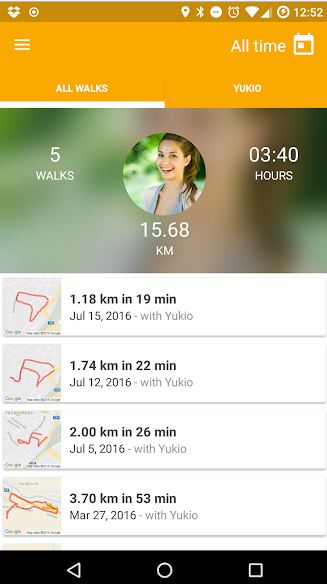
\includegraphics[scale=0.3]{21dogwalk}
     \caption{Dog Walk}
\end{figure}
\section{My Pet Reminders\cite{capseven}}
My pet Reminder is mobile base application for android and IOS mobile user. This is useful in making a pet profile, generating a reminder of pet important dates for example birthday or appointment but the pet diet, diseases, treatment suggestions and healthcare services functionalities are not the part of this application currently.
\begin{figure}[H]
  \centering
    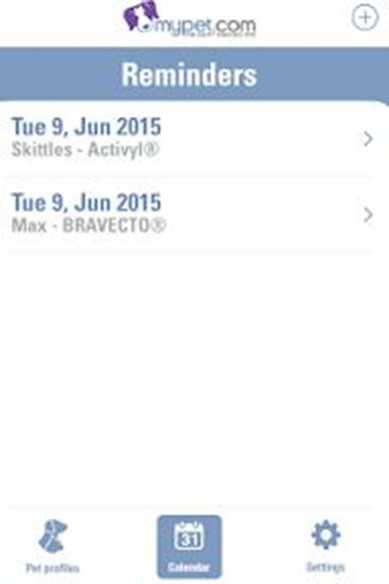
\includegraphics[scale=0.3]{22MyPetRemainder}
     \caption{My Pet Reminders}
\end{figure}
\section{Dog Sync\cite{capseight}}
It is web portal. This is very useful application in recording pet activities for example when the pet watered, when the pet walked, when the medicine is given and when the pet is fed. User can also share this record with the friends and other users of this application. This web application lacks the pet diet plans and diseases details and some other necessary healthcare services. This application is limited to only dogs. Android version and IOS version of this application is currently not available.
\begin{figure}[H]
  \centering
    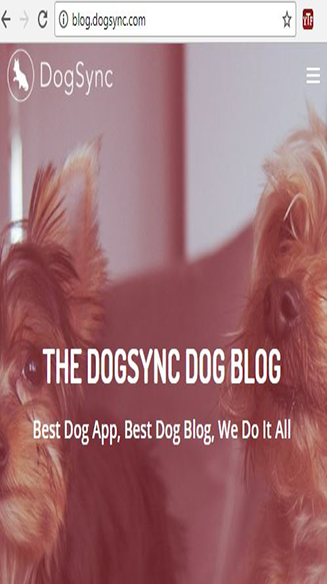
\includegraphics[scale=0.3]{23DogSync}
      \caption{Dog Sync}
\end{figure}
\section{ASPCA Pet Safety\cite{capsnine}}
The ASPCA has multiple applications for the pet owners regarding safety and locating the pet in case the pet is lost. The ASPCA Pet Safety app is available for both Android, IOS users. this application can help pet owners plan for pet safety during emergencies, natural disasters and extreme weather. The app teaches safety and preparedness hints, it also suggestions on how to search for lost pets right after emergencies and tools for storing pet information or creating a lost pet kit. The drawback of using this application is that it does not provide important functionality like, this application does not provide any monitoring of the health of the pet. It does not provide access to a vet for appointment and checkups.
\begin{figure}[H]
  \centering
    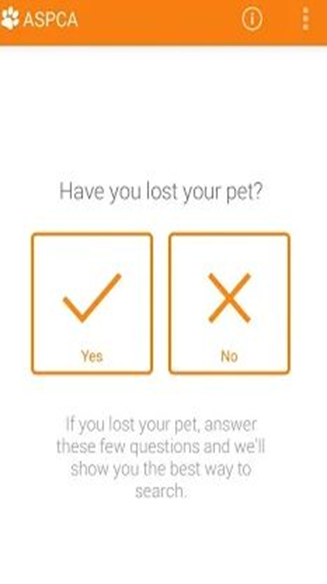
\includegraphics[scale=0.3]{24ASPCAapp}
      \caption{ASPCA Pet Safety}
\end{figure}
\section{Dog Health[9]}
This app is used because it generates  reminders about the appointments with your vet. The drawback of this application is that this application does not keeps track of the previous visits to the vet  and does not store any medication administration that has to be done. Overall this application is very is not useful.The only function that  this application performs is generating alerts.
\begin{figure}[H]
  \centering
    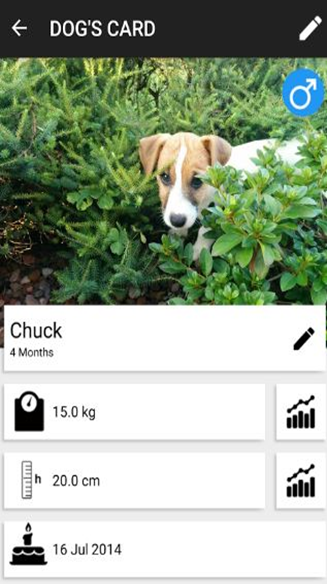
\includegraphics[scale=0.3]{25Doghealth}
     \caption{Dog Health}
\end{figure}
\section{Pet Coach\cite{petcoach}}
Pet coach is a complete platform for the web, android and IOS users. The application generates the advices and tips for pet’s health from the professional pet doctors. After installing this application anyone can post the question related to his pet diet, behavior and training. Consultations are free and well as paid for the users. Although pet coach is a very useful application but this is limited to take an appointment or advises from the doctor. While weekly and daily diet plan, pet common diseases, treatment plan and notifications features are considered as out of scope now.
\begin{figure}[H]
  \centering
    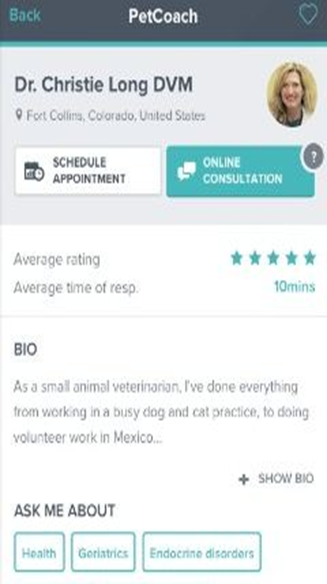
\includegraphics[scale=0.3]{26petcoach}
      \caption{Pet Coach}
\end{figure}
\section{Pet-First Aid\cite{petfirstage}}
Pet-First Aid based upon a very unique idea by American android and IOS developer Red Cross. Application includes the photos, videos, tips and first aid guidelines in case of emergency or injury. If the injury of the pet is very severe then the application can view the hospital list located nearby or contact the pet doctor. While using this application user can’t view the diet plan, common diseases, treatment plan and notification features.
\begin{figure}[H]
  \centering
    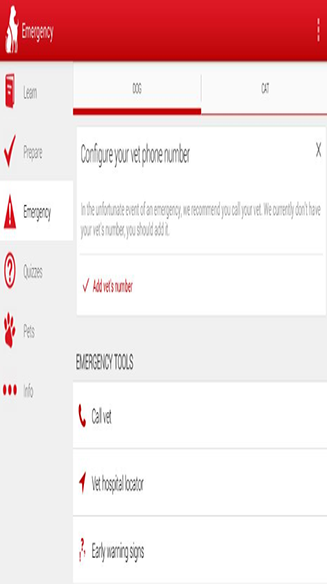
\includegraphics[scale=0.3]{27petfirstaid}
    \caption{Pet-First Aid}
\end{figure}
\section{Rover\cite{capsrover}}
Rover is complete platform web, android and IOS users.  It basically establishes the network of such persons who are dog owner. Dog owners usually find too much difficulty in finding the sitters and boarding. This application is limited to provide facility to the dog owners in booking sitters for their dogs for boarding purpose, finding dogs care center, and send notifications to the pet users related to the updated photos of home sittings. Although this is very useful but confined to the dogs day care centers and homes. 
\begin{figure}[H]
  \centering
    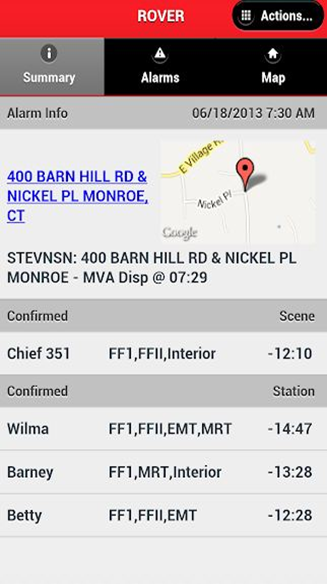
\includegraphics[scale=0.3]{28rover}
      \caption{Rover}
\end{figure}
There are many mobile applications which are related to pets but few are discussed in details. Most of them work on the specific single feature; for example Rover is an application which helps in searching the dog day care centers. Pet First Aid helps in searching out the pet hospitals in case of emergency. Pet Coach helps in taking out the advises and tips from the professional pet doctor. Dog Health is confined to the dog health only. ASPCA Pet Safety helps the pet owners in the case of pet loss. Dog walk is limited to record the walk and activities of dog. My Pet Remainder helps to notify the owner related to important dates of his pet like birthday etc. “Pet Diet and Health care Planner is focusing on many features like generate pet diet plan, diseases details, generate alarm  notification on pet food time and take an appointment.









\chapter{Requirement Specifications} \label{chap:reqs}

%\version{v1.10.2015}

\section{Existing System}
Currently, there is no online system which is being used by the Islamabad Pet & AVIAN Hospital G-10/4. Currently they are using manual system. No website and android application is still being used by the hospital.
\section{Proposed System}
Layman who buys the pet does not know the proper diet plans, their common diseases, treatment suggestions and sometime forget to fed . Pet Diet and Health care planner is an industrial project and it is designed and developed for the Islamabad Pets & AVIAN Hospital. It is a complete platform. The android application will support the user in generating pet diet plans, notify the owner on the proper timings that when your pet need food and also provide the pet disease and treatment suggestions. Users can take the appointment through android application and as well as through website. Website user can view information like hospital services etc as per as hospital requirement.

\section{Requirement Specification}
Requirements specification includes functional and as well as non functional requirements.
\subsection{Functional Requirements}
\begin{enumerate}[label=\alph*]
\item. Functional Requirement 1 (Registration)
Description:
Registration is compulsory for everyone who is using the Android Application for the first time. Registration will be perform to ensure the user account.
\item. Functional Requirement 2 (Login)
Description:
After the successful registration user is able to log in into the Android Application through the already registered email and password.
\item. Functional Requirement 3 (Add / View Pet Profile Details)
Description:
Android Application user can add and view the pet profiles. 
\item. Functional Requirement 3 (View/ Download Details)
Description:
Android Application user can view and download the diet plans and diseases details and treatment details. 
\item. Functional Requirement 3 (Generate Notification)
Description:
Application user can generate the alarm notification so that pet feed on proper timing.	
\item. Functional Requirement 3 (Take an Appointment)
Description:
Users can take the appointment through Android Application and as well as through website.
\item. Functional Requirement 5 (Website Application)
Description: 
Website user can take an appointment and view information like hospital services etc as per as hospital requirements.
\item. Functional Requirement 6 (Add as a Doctor)
Description: 
Android admin able to register doctor if assigned hospital id matches with the entered id.
\item. Functional Requirement 7(Logout)
Description:
Application users can logout at any time.
\end{enumerate}

\subsection{ Subsystem Functional Requirement}
\begin{enumerate}[label=\alph*]
\item. Login Processing
Description
Login activity is being performed on the system.
\item. Validation Check
Description
While log in into the system; system will perform validation either the email or password is correct or not.
\end{enumerate}

\subsection{Non Functional Requirement}
\begin{enumerate}[label=\alph*]
\item.	Performance
Least specification constraint is performed by the personal computer and which is necessary for every platform like android or web application. Memory, processor and operation system should match with the application.
\item.	Accuracy
If the application display the correct results like application is fetching correctly the pet diseases or treatment details etc according to user choice,  at run time then the application will be accurate.
\item.	Maintainability
The developer will perform the maintenance of both applications; android as well as web application if some issue occur.
\item.	Portability
It is true that now a day’s users demand the portable applications. Pet Diet and Healthcare is portable because it is available on both platforms android and as well as web.
\item.	Availability	
Application user is capable to perform and view application details on any time.
\item.	Flexibility
Pet diet and Healthcare planner is fully compatible and flexible system and easy to use for the end users.
\item.	Usability
The interface and Graphical User Interface design of the application is user friendly with no training required.
\end{enumerate}
\newpage
\section{Use Cases}
Uses case diagrams are very important because they help in understanding the whole system in a shorter time or quickly. Use case diagrams are designed for the both platforms android as well as for the web site.
\section{Use Case (System Diagram)}
Website user can view the information and make an appointment through website. 
Android Application user or pet owner can register then login into the system. After logging into the system the user can generate pet diet plan, view diseases details, add/view pet profiles, Add/view/delete food timings notification alarm, take/cancel appointment and log out.

\begin{figure}[H]
    \centering
    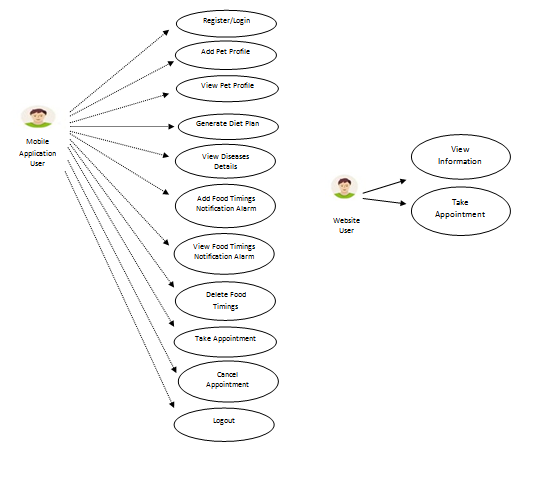
\includegraphics[scale=0.7]{301}
		\caption{Use Case (System Diagram)}
\end{figure}

\newpage
\subsection{Use Case (Website User)}
\begin{figure}[H]
  \centering
    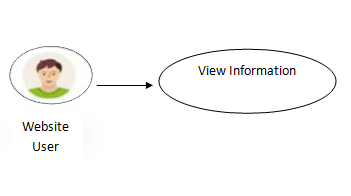
\includegraphics{42UseCase}
		\caption{View Information}
\end{figure}
Website user can view the every information which is provided by the pet hospital like services etc.
\begin{table}[ht]
\centering

\label{View Information (website)}
\begin{tabular}{|l|l|}
\hline
Name                     & View Information(website)                                                                                                                                        \\ \hline
Actor                    & Website user                                                                                                                                                     \\ \hline
Brief Description        & \begin{tabular}[c]{@{}l@{}}Website user is able to view the every information which\\  is mentioned on the website.\end{tabular}                                 \\ \hline
Flow of Events           & \begin{tabular}[c]{@{}l@{}}User can view hospital services, about us and doctors \\ detail etc or any further information provided by the hospital.\end{tabular} \\ \hline
Alternate Flow of Events & User will take an appointment.                                                                                                                                   \\ \hline
Pre-condition            & \begin{tabular}[c]{@{}l@{}}Should click on any button in the menu bar or scroll down\\ the cursor.\end{tabular}                                                  \\ \hline
Post condition           & User might take a decision of appointment.                                                                                                                       \\ \hline
\end{tabular}
\caption{View Information (website)}
\end{table}


\newpage
\begin{figure}[H]
  \centering
    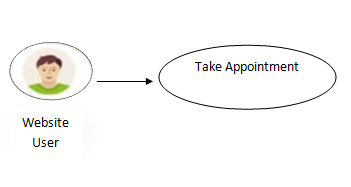
\includegraphics{43UseCase}
     \caption{Appointment (website)}
\end{figure}
By using the website feature our users will be able to take appointments online.
\begin{table}[ht]
\centering
\label{Appointment (website)}
\begin{tabular}{|l|l|}
\hline
Name                      & Appointment(website)                                                                                                                                                            \\ \hline
Actor                     & Website user                                                                                                                                                                    \\ \hline
Brief Description         & Website user is able to take an appointment.                                                                                                                                    \\ \hline
Flow of Events            & \begin{tabular}[c]{@{}l@{}}User will fill all the inputs text fields required for taking an\\ appointment. Like enter mobile number, pet name, date and times etc.\end{tabular} \\ \hline
Alternate Flow of  Events & User will view the information.                                                                                                                                                 \\ \hline
Pre-condition             & Fill all the input text fields.                                                                                                                                                 \\ \hline
Post condition            & Response email will be send to the user.                                                                                                                                        \\ \hline
\end{tabular}
\caption{Appointment (website)}
\end{table}




\newpage
\subsection{Use Case (Android User)}
\begin{figure}[H]
    \centering
    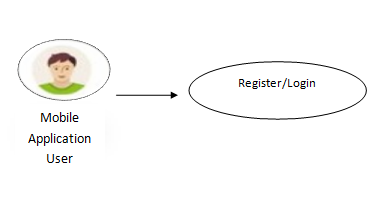
\includegraphics{31UseCase}
		\caption{Registrations/ Login}
\end{figure}
First of all Android Application User will register himself by filling registration form in order to login into the system or perform other activities.
\begin{table}[ht]
\centering

\label{Registrations/ Login}
\begin{tabular}{|l|l|}
\hline
Name                      & Registration/ Login                                                                                                                                                                                                                                                                   \\ \hline
Actor                     & Android Application User                                                                                                                                                                                                                                                              \\ \hline
Brief Description         & Registration is compulsory for the first time to login.                                                                                                                                                                                                                               \\ \hline
Flow of Events            & \begin{tabular}[c]{@{}l@{}}Fill all the input text fields.Provided information will be verified \\ then user will be register. If user is already register then there is no\\ need of performing registration. Registration is compulsory\\ for the first time to login.\end{tabular} \\ \hline
Alternate Flow of  Events & If validation fails, then user can resend it.                                                                                                                                                                                                                                         \\ \hline
Pre-condition             & All fields of registration and login are essential.                                                                                                                                                                                                                                   \\ \hline
Post condition            & User will login into the system and perform other activities.                                                                                                                                                                                                                         \\ \hline
\end{tabular}
\caption{Registrations/ Login}
\end{table}



\newpage
\begin{figure}[H]
  \centering
    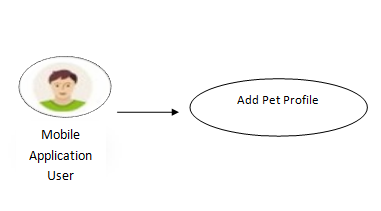
\includegraphics{32UseCase}
     \caption{Add Pet Profile}
\end{figure}
Android Application User can add pet profile details upon successful login.
\begin{table}[ht]
\centering

\label{Add Pet Profile}
\begin{tabular}{|l|l|}
\hline
Name                      & Add Pet Profile                                                                                                                                         \\ \hline
Actor                     & Android Application User                                                                                                                                \\ \hline
Brief Description         & User is able to add the pet profiles.                                                                                                                   \\ \hline
Flow of Events            & \begin{tabular}[c]{@{}l@{}}Fill the all input text fields necessary for the pet profile\\ then added profiles are saved into the database.\end{tabular} \\ \hline
Alternate Flow of  Events & If fields are missing then user can refill them.                                                                                                        \\ \hline
Pre-condition             & Some information is necessary                                                                                                                           \\ \hline
Post condition            & Added information can be viewed.                                                                                                                        \\ \hline
\end{tabular}
\caption{Add Pet Profile}
\end{table}




\newpage
\begin{figure}[H]
  \centering
    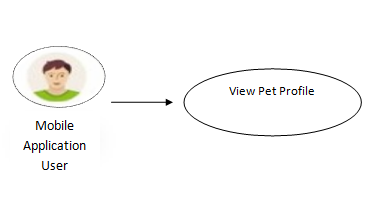
\includegraphics{33UseCase}
      \caption{View Pet Profile}
\end{figure}
Android Application User can also view the pet profile.
\begin{table}[ht]
\centering

\label{View Pet Profile}
\begin{tabular}{|l|l|}
\hline
Name                      & View Pet Profile                                                                                                       \\ \hline
Actor                     & Android Application User                                                                                               \\ \hline
Brief Description         & User is able to view the pet profile fetched from the databases.                                                       \\ \hline
Flow of Events            & \begin{tabular}[c]{@{}l@{}}After clicking the view profile button user is able to view the pet\\ profile.\end{tabular} \\ \hline
Alternate Flow of  Events & If click on any other button.                                                                                          \\ \hline
Pre-condition             & If view profile button is clicked.                                                                                     \\ \hline
Post condition            & Viewed information is fetched from database.                                                                           \\ \hline
\end{tabular}
\caption{View Pet Profile}
\end{table}





\newpage
\begin{figure}[H]  
  \centering
    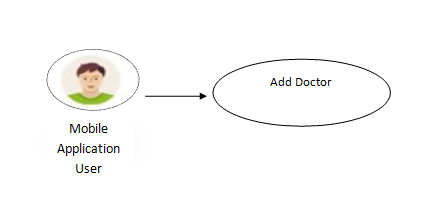
\includegraphics{45UseCase}
    \caption{Add Doctor Profile}
\end{figure}
Admin can register as a doctor if and only if the entered hospital id matches with the assigned hospital id.

\begin{table}[ht]
\centering
\label{Add Doctor Profile}
\begin{tabular}{|l|l|}
\hline
Name                      & Add Doctor                                                                                                                                           \\ \hline
Actor                     & Android Application User                                                                                                                             \\ \hline
Brief Description         & User is able to add himself as a doctor if and only if the hospital id matches.                                                                      \\ \hline
Flow of Events            & \begin{tabular}[c]{@{}l@{}}Fill the all input text fields necessary for the  profile then added profiles are\\ saved into the database.\end{tabular} \\ \hline
Alternate Flow of  Events & If fields are missing then user can refill them.                                                                                                     \\ \hline
Pre-condition             & Some information is necessary                                                                                                                        \\ \hline
Post condition            & Added information can be viewed.                                                                                                                     \\ \hline
\end{tabular}
\caption{Add Doctor Profile}
\end{table}



\newpage
\begin{figure}[H]
  \centering
    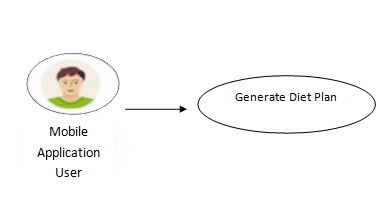
\includegraphics{34UseCase}
     \caption{Generate and Download Diet Plan}
\end{figure}
Android Application User can also generate and download the pet diet plan. Diet plans are generated on the basis of pet specie, breed(weekly or daily) ,age and type of plan.
\begin{table}[ht]
\centering

\label{Generate and Download Diet Plan}
\begin{tabular}{|l|l|}
\hline
Name                                      & View / Download Diet Plan                                                                                                                                                                             \\ \hline
Actor                                     & Android Application User                                                                                                                                                                              \\ \hline
Brief Description                         & User is able to view and download the pet diet plan.                                                                                                                                                  \\ \hline
Flow of Events                            & \begin{tabular}[c]{@{}l@{}}Select the pet specie, breed, age and type of plan (weekly or daily) then click\\ on generate plan button then diet plan will be generated from the database.\end{tabular} \\ \hline
\multirow{2}{*}{Alternate Flow of Events} & \multirow{2}{*}{If any filed is missing then no plan will be shown and downloaded.}                                                                                                                   \\
                                          &                                                                                                                                                                                                       \\ \hline
Pre-condition                             & If generate or download diet plan button is clicked.                                                                                                                                                  \\ \hline
Post condition                            & Information is fetched from database.                                                                                                                                                                 \\ \hline
\end{tabular}
\caption{Generate and Download Diet Plan}
\end{table}




\newpage
\begin{figure}[H]
  \centering
    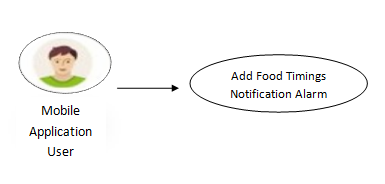
\includegraphics{36UseCase}
     \caption{Add Notificationn Alarm}
\end{figure}
Application User can add notification alarm for the multiple pets.
\begin{table}[ht]
\centering

\label{Add Notificationn Alarm}
\begin{tabular}{|l|l|}
\hline
Name                                      & Add\View Notification Alarm                                                                                                                            \\ \hline
Actor                                     & Android Application User                                                                                                                          \\ \hline
Brief Description                         & \begin{tabular}[c]{@{}l@{}}User is able to add and view the notification alarm related to\\ pet food timings for the multiple pets.\end{tabular}           \\ \hline
Flow of Events                            & \begin{tabular}[c]{@{}l@{}}Set the alarm time and then enter the pet name.\\ Then click on set alarm button. Alarm will be set down.\end{tabular} \\ \hline
\multirow{2}{*}{Alternate Flow of Events} & \multirow{2}{*}{User can delete any list item.}                                                                                                   \\
                                          &                                                                                                                                                   \\ \hline
Pre-condition                             & Pet name, time and click on set alarm button are necessary.                                                                                       \\ \hline
Post condition                            & Alarm can be deleted.                                                                                                                             \\ \hline
\end{tabular}
\caption{Add Notificationn Alarm}
\end{table}



\newpage
\begin{figure}[H]
  \centering
    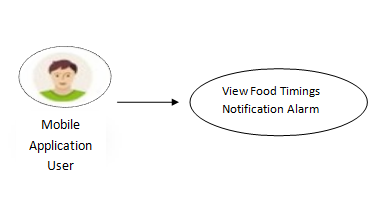
\includegraphics{37UseCase}
    \caption{View Notification List}
\end{figure}
Application User can also view the all information available on application related to notifications of pet food timings.
\begin{table}[ht]
\centering

\label{View Notification List}
\begin{tabular}{|l|l|}
\hline
Name                     & View Notification List                                                          \\ \hline
Actor                    & Android Application User                                                        \\ \hline
Brief Description        & User is able to view the notification list related to pet food timings.         \\ \hline
Flow of Events           & Click on Alarm list then user will be able to view the notification alarm list. \\ \hline
Alternate Flow of Events & User can delete any list item.User can turn off the alarm.                      \\ \hline
Pre-condition            & Click on alarm list button is necessary.                                        \\ \hline
Post condition           & Viewed information can be deleted.                                              \\ \hline
\end{tabular}
\caption{View Notification List}
\end{table}


\newpage
\begin{figure}[H] 
  \centering
    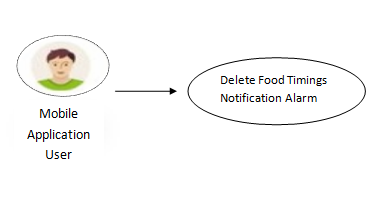
\includegraphics{38UseCase}
    \caption{Delete Notification Alarm}
\end{figure}
Application User can delete the notification list items one by one.
\begin{table}[ht]
\centering

\label{Delete Notification Alarm}
\begin{tabular}{|l|l|}
\hline
Name                     & Delete Notification Alarm                                                                                                                                         \\ \hline
Actor                    & Android Application User                                                                                                                                          \\ \hline
Brief Description        & User is able to delete the any notification list item related to pet food timings.                                                                                \\ \hline
Flow of Events           & \begin{tabular}[c]{@{}l@{}}Click on Alarm list then click on cross sign; a dialog box will be opened if yes\\ is clicked then alarm will be deleted.\end{tabular} \\ \hline
Alternate Flow of Events & User can turn off any alarm.                                                                                                                                      \\ \hline
Pre-condition            & If yes in clicked.                                                                                                                                                \\ \hline
Post condition           & Can perform on other activities or add a new alarm.                                                                                                               \\ \hline
\end{tabular}
\caption{Delete Notification Alarm}
\end{table}


\newpage
\begin{figure}[H]
  \centering
    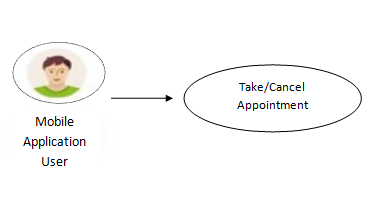
\includegraphics{46UseCase}
      \caption{Take / Cancel Appointment}
\end{figure}
Android Application user is able to take an appointment or cancel it. 
\begin{table}[ht]
\centering

\label{Take / Cancel Appointment}
\begin{tabular}{|l|l|}
\hline
Name                     & Take / Cancel  Appointment                                                                                                                                                               \\ \hline
Actor                    & Android Application User                                                                                                                                                                 \\ \hline
Brief Description        & Emails will send for the both cases if appointment is taken or cancelled.                                                                                                                \\ \hline
Flow of Events           & \begin{tabular}[c]{@{}l@{}}If appointment button is clicked then appointment email will be send.\\ If cancel button is clicked then cancel the appointment message is send.\end{tabular} \\ \hline
Alternate Flow of Events & User can view the doctors’ information.                                                                                                                                                  \\ \hline
Pre-condition            & If appoint or cancel button in clicked.                                                                                                                                                  \\ \hline
Post condition           & Can perform other activities within the application...                                                                                                                                   \\ \hline
\end{tabular}
\caption{Take / Cancel Appointment}
\end{table}


\newpage
\begin{figure}[H]
  \centering
    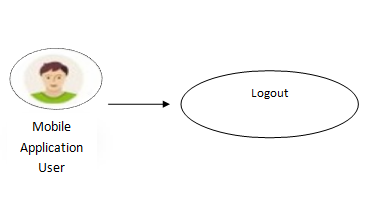
\includegraphics{41UseCase}
  \caption{Logout Details Specification}
\end{figure}

Application User is able to logout at any time.
\begin{table}[ht]
\centering

\label{Logout Details Specification}
\begin{tabular}{|l|l|}
\hline
Name                     & Logout                                                                 \\ \hline
Actor                    & Android Application User                                               \\ \hline
Brief Description        & After successful login Application User is able to logout at any time. \\ \hline
Flow of Events           & Click on logout button then user will be logout from the application.  \\ \hline
Alternate Flow of Events & Shut down the system.                                                  \\ \hline
Pre-condition            & All activates are completed no more need to stay log in.               \\ \hline
Post condition           & User is able to re login into the system at any time.                  \\ \hline
\end{tabular}
\caption{Logout Details Specification}
\end{table}


















\chapter{System Design} \label{chap:design}

%\version{v1.10.2015}

\section{System Architecture Diagram}
System Architecture Diagram is a theoretic model that defines the overall view of a system. In architecture diagram we basically have defined the whole structure of a system. Android user can login/register using android application and can add and view any details like add pet profile, view pet profile, generate diet plan, alarm notification details and appointment. Added information is saved into the database and fetched from the database. While can view the information displayed on the website. Appointments can be taken through android and as well as through website user. The system architecture diagram is given below:

\begin{figure}[H]
\centering
   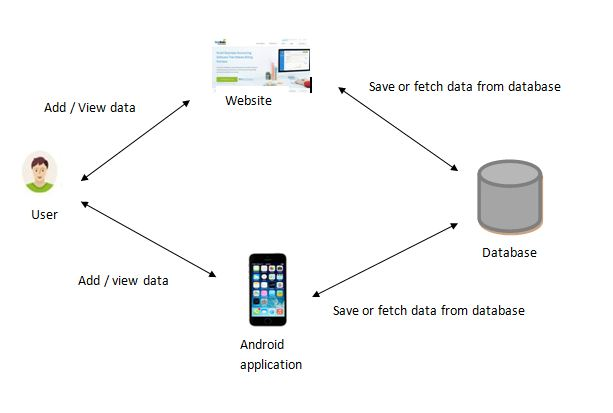
\includegraphics[scale=0.7]{4chap}
    \caption{System Architecture Diagram}
\end{figure}

\newpage
\section{Design Methodology}
Agile methodology is used to develop this project as; our requirements are incremental.

\begin{figure}[H]
  \centering
    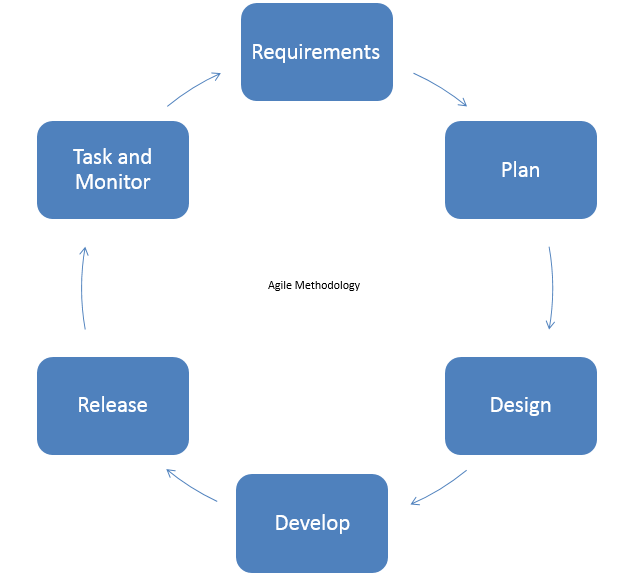
\includegraphics[scale=0.6]{Designmethod}
     \caption{Design Methodlogy}
\end{figure}



\newpage
\section{High Level Deign}
High level designs include flow charts and activity diagrams of the website and android application.

\subsection{Flow Chart}
\begin{enumerate}
\item \textbf{Flow Chart (website user)}\\
Website user first of all; will login into the system. If email and password is correct then user can only view the details available on the web application or take an appointment run time.

\begin{figure}[H]
\centering
  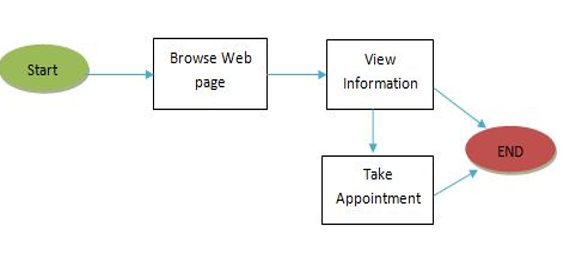
\includegraphics[scale=0.5]{figflow}
  \caption{Flow Diagram of a system (Website user)}
\end{figure}

\item \textbf{Flow Chart (Android Application user)}
\\ First of all android user will login into the system if the email and password is correct then android will be able to view details. User can add, delete and update data which is specific to pet profile. Changes in pet profile will be saved and he can fetch and re view them. Android user can take appointment or contact the doctor in case of   any emergency. Android user can log out at any time.

\begin{figure}[H]
    \centering
    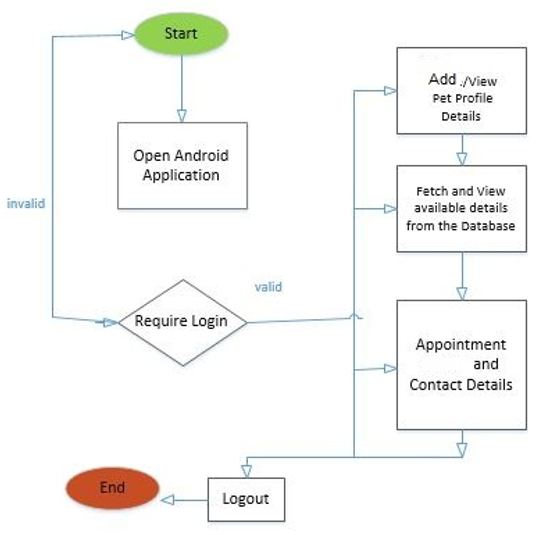
\includegraphics[scale=0.5]{figflowtwo}
    \caption{Flow Diagram of a system (Android Application User)}
\end{figure}
\end{enumerate}


\newpage
\subsection{Activity Diagrams}

\item \textbf{Activity Diagram (website user)}\\
Web user can view the details available on the web application or take an appointment at any time.
\begin{figure}[H]
\centering
   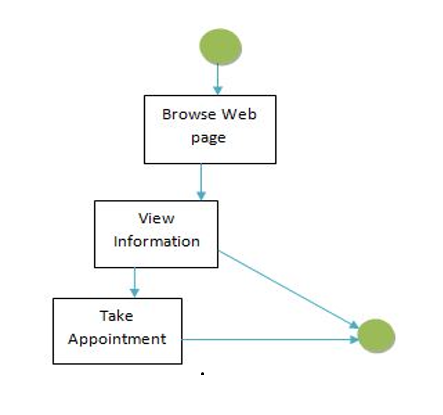
\includegraphics[0.3]{actone}
    \caption{Activity Diagram for a web user}
\end{figure}
\newpage
\item \textbf{Activity Diagram (Android Application user)}\\
\begin{figure}[H]
\centering
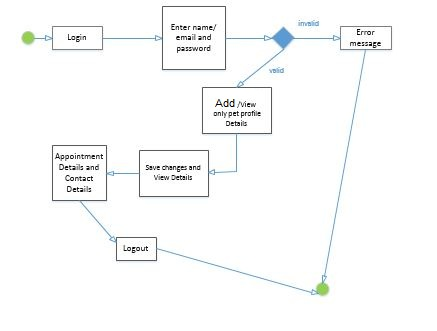
\includegraphics[0.3]{acttwo}
  \caption{Activity Diagram for an Android app user}
\end{figure}
First of all android user will login into the system if the email and password is correct then android will be to view details. User can add and view data which is specific to pet profile. User can view and generate and download the diet plans and diseases details. Android user can take appointment or contact the doctor in case of   any emergency. Android user can log out at any time.

\newpage
\item \textbf{ER Diagram)}\\
User can generate pet diet plans by selecting the correct pet specie,breed and age.User can also take an appointment and add multiple pets.User is able to view pet diseases details. 

\begin{figure}[H]
\centering
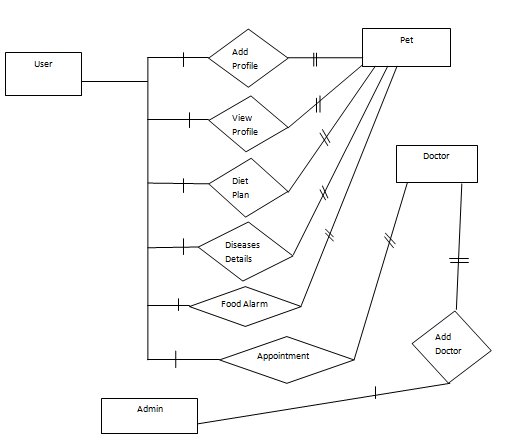
\includegraphics[0.3]{ERD}
  \caption{Activity Diagram for an Android app user}
\end{figure}









\chapter{System Implementation} \label{chap:sysImplementation}
%\version{v1.10.2015}

\section{System Architecture}
Pet Diet and Health care planner consists of android application and as well as web application. The android application will generate the pet diet plan, pet diseases details, diet notification alarm and doctor appointment. Pet diet plans are saved into the cloud base database and that are retrieve on the basis of pet age, specie and kind of breed. Diseases details will be shown on the basis of pet specie.\par Notification alarm will be generated on the proper timings within a day. Email will send on time when the user click on the appointment button in android application. The web application will display the hospital information like hospital services and doctors.

\section{Tools and Technology Used}
\begin{enumerate}
\item \textbf{Microsoft office}\\Microsoft office is used for project documentation and presentation. Microsoft Visio is useful for designing flow charts, activity and system diagrams.
\item \textbf{Adobe Photoshop for designing}\\Adobe photo shop is very helpful for designing the mobile application layouts, compressing the images size and increasing the resolution.
\item \textbf{Canva online designing tool}\\Canva is the online tool for graphics. The tool has been used for shades and image transparency.
\end{enumerate}


\subsection{Developers Tools}
\begin{enumerate}
\item \textbf{Android studio 3.0.1}\\
Currently the most stable version of android studio is android studio 3.0.1. Provide many facilities like latest use of libraries and API’s.
\item \textbf{Firebase  database}\\
Firebase is GOOGLE supported Cloud base platform. It is highly flexible and responsive. Providing user authentication, storage and hosting etc.
\item \textbf{Sublime Text3}\\
Sublime Text3 tool is used in developing web pages.
\end{enumerate}
\subsection{Languages Used}
\begin{enumerate}
\item \textbf{html, css, bootstrap }
      Web application is developed under html, css, and bootstrap and java script.
\item \textbf{Java}
      Android mobile application support java.
\item \textbf{Xml}
     Android studio support XML for designing application layouts or mockups.
\item \textbf{html, css, bootstrap }
      Web application is developed under html, css, and bootstrap and java script.
\item \textbf{Java}
      Android mobile application support java.
\item \textbf{Xml}
     Android studio support XML for designing application layouts or mockups.
\end{enumerate}

\section{Processing Logic}
Firstly user will login into the android app then user can view the main home activity. User can input the information related to pet specie, breed and age and then view the detail which is generated by the firebase database. User can generate the food timing notification alarm to feed his/her pet on time. Appointment can be taken through android and as well as through the website user.
\begin{figure}[H]
\centering
  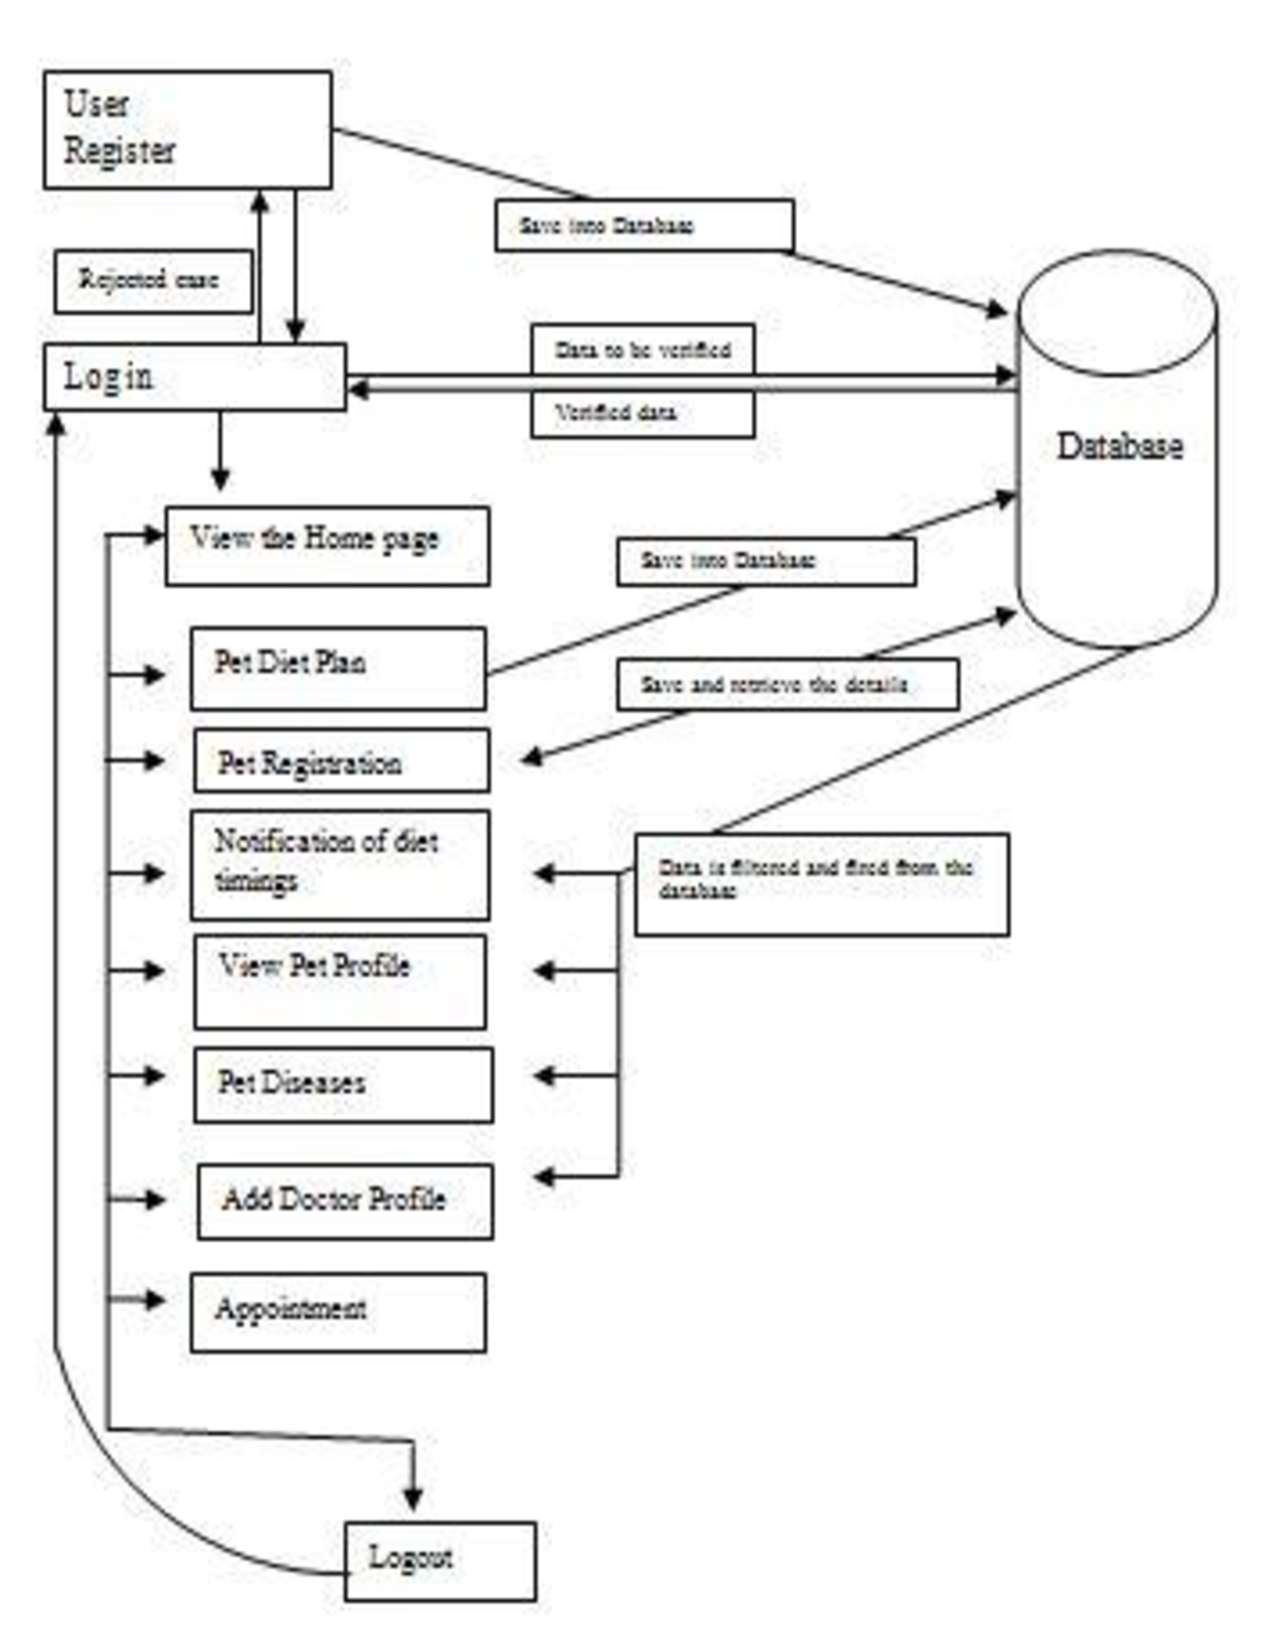
\includegraphics[scale=0.5]{fivethree}
  \caption{Activity Processing Logic}
\end{figure}
Website will only display the data which is provided by the Islamabad Pets & AVIAN Hospital G-10/4 sector. Website will handle and full fill the requirements of the hospital. Currently the website is displaying the Hospital information, services, doctors details and appointment facility.

\section{Application Access Security}
Cloud base database (firebase) which provides many services like secure authentication, push notification, cloud messaging, remote access, real time database etc. Security reasons, fast access and the reliable user authentication firebase database; used for this android project. Recently Gmail authentication is used for the user login in; later on other authentication methods might be used for the user access. 
\subsection{Database Security}
Firebase is a real time database which has separate security rules for user authentication, database and for the storage access. 

Database security rules are shown in below picture.

\begin{figure}[H]
 \centering
  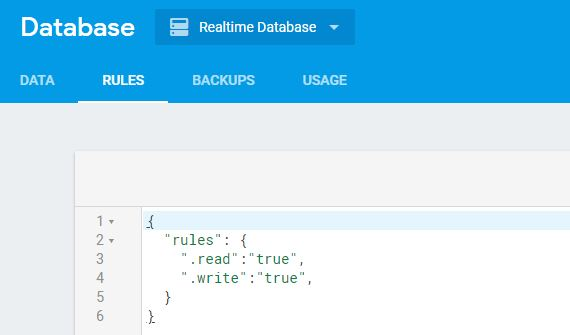
\includegraphics[scale=0.3]{asd}
  \caption{Firebase Database}
\end{figure}
	
Storage security rules are shown in below picture.
\begin{figure}[H]
\centering
 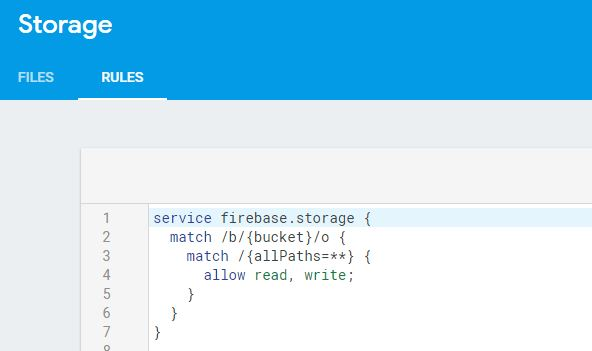
\includegraphics[scale=0.3]{dfg}
  \caption{Firebase Storage}
\end{figure}
Data is stored in the form of nodes into the JSON format. Unique keys or ids are created against each record. Security rules and creation of unique keys is a very handsome feature of firebase which make it different from other in aspect of authentication and database security.
\chapter{System Testing and Evaluation}\label{chap:testingEvaluation}

\section{Test Cases}
Testing is extremely important, both to ensure that the system meets requirements and to ensure that it is free of errors. That is why it is performed throughout the development process at every level.

\subsection{User Authentication}

\begin{table}[ht]
\centering
\label{User Authentication}
\begin{tabular}{|l|l|}
\hline
Test Case ID                      & Test 1                                                                                                                     \\ \hline
Objective                         & Verify Registration/ login activity.                                                                                       \\ \hline
Environment                       & Android Application                                                                                                        \\ \hline
Prerequisite                      & Application must run.                                                                                                      \\ \hline
Method                            & \begin{tabular}[c]{@{}l@{}}1. Enter Valid email.\\ 2. Enter Valid Password.\\3. Click on Register/Login button.\end{tabular} \\ \hline
Expected Results                  & After successful verification user is able to login.                                                       \\ \hline
Verification should be performed. & Pass                                                                                                                       \\ \hline
\end{tabular}
\caption{User Authentication}
\end{table}	
Enter valid email, password and then click on login button for verification. If user is not register then enter email, password and phone for registration.  After successful verification user is able to login into the system.

	
\newpage
\subsection{Add Pet Profile}
\begin{table}[ht]
\centering
\label{Add Pet Profile}
\begin{tabular}{|l|l|}
\hline
Test Case ID                         & Test 2                                                                                                             \\ \hline
Objective                            & Pet profiles details should be added into the database.                                               \\ \hline
Environment                          & Android Application                                                                                                \\ \hline
Prerequisite                         & Application must run.                                                                                              \\ \hline
Method                               & \begin{tabular}[c]{@{}l@{}}1- Fill the all the input text fields properly.\\ 2- Click on save button.\end{tabular} \\ \hline
Expected Results                     & Should save into the database successfully.                                                                        \\ \hline
Database  updated successfully. & Pass                                                                                                               \\ \hline
\end{tabular}
\caption{Add Pet Profile}
\end{table}

Fill all the input fields properly then click on save button to upload data. Data base should be updated successfully.


\newpage
\subsection{Add Doctor Profile}
\begin{table}[ht]
\centering
\label{Add Doctor Profile}
\begin{tabular}{|l|l|}
\hline
Test Case ID                         & Test 3                                                                                                                                                                      \\ \hline
Objective                            & Doctor profiles details should be added into the database.                                                                                                     \\ \hline
Environment                          & Android Application                                                                                                                                                         \\ \hline
Prerequisite                         & Application must run.                                                                                                                                                       \\ \hline
Method                               & \begin{tabular}[c]{@{}l@{}}1- Fill the all the input text fields properly.\\ 2- Enter correct hospital id assigned by the hospital.\\ 3- Click on save button.\end{tabular} \\ \hline
Expected Results                     & Should save into the database successfully.                                                                                                                                 \\ \hline
If database is updated successfully. & Pass                                                                                                                                                                        \\ \hline
\end{tabular}
\caption{Add Doctor Profile}
\end{table}
Fill the all the input text fields properly. Enter correct hospital id assigned by the hospital. Click on save button. Data base should be updated successfully.
	
\newpage
\subsection{View Pet Profile}
\begin{table}[ht]
\centering
\label{View Pet Profile}
\begin{tabular}{|l|l|}
\hline
Test Case ID                        & Test 4                                                       \\ \hline
Objective                           & To view to pet profile.                                       \\ \hline
Environment                         & Android Application                                           \\ \hline
Prerequisite                        & Application must run.                                         \\ \hline
Method                              & 1- Click on View profile button.                              \\ \hline
Expected Results                    & Pet profile of the pet owner should be fetched from the database. \\ \hline
If profile is successfully fetched. & Pass                                                          \\ \hline
\end{tabular}
\caption{View Pet Profile}
\end{table}	
Click on View profile button.  Pet profile should be fetched from the database.

\newpage
\subsection{Generate pet Diet Plan}
\begin{table}[ht]
\centering
\label{Generate pet Diet Plan}
\begin{tabular}{|l|l|}
\hline
Test Case ID                        & Test 5                                                                                                           \\ \hline
Objective                           & Diet plan should be fetched successfully.                                                                        \\ \hline
Environment                         & Android Application                                                                                              \\ \hline
Prerequisite                        & Application must run.                                                                                            \\ \hline
Method                              & \begin{tabular}[c]{@{}l@{}}1- Select pet specie, breed and age.\\ 2- Click on Generate Plan button.\end{tabular} \\ \hline
Expected Results                    & Pet diet plan should be fetched from database successfully.                                                          \\ \hline
If successfully fetch from database & Pass                                                                                                             \\ \hline
\end{tabular}
\caption{Generate pet Diet Plan}
\end{table}
Select pet specie, breed and age. Click on Generate Plan button.  Diet plan should be fetched from database.

\newpage
\subsection{View Pet Diseases Detail}
\begin{table}[ht]
\centering
\label{View Pet Diseases Detail}
\begin{tabular}{|l|l|}
\hline
Test Case ID                        & Test 6                                                                                                               \\ \hline
Objective                           & \begin{tabular}[c]{@{}l@{}}Common diseases details of pets should be fetched from the \\ database successfully.\end{tabular} \\ \hline
Environment                         & Android Application                                                                                                  \\ \hline
Prerequisite                        & Application must run.                                                                                                \\ \hline
Method                              & \begin{tabular}[c]{@{}l@{}}1-Select pet specie.\\ 2-Click on View Details button.\end{tabular}                       \\ \hline
Expected Results                    & Details should be fetched from database successfully.                                                                \\ \hline
If successfully fetch from database & Pass                                                                                                                 \\ \hline
\end{tabular}
\caption{View Pet Diseases Detail}
\end{table}
Select pet specie. Click on View Details button.  Details should be fetched from database.

\newpage
\subsection{Notification Alarm}
\begin{table}[ht]
\centering
\label{Notification Alarm}
\begin{tabular}{|l|l|}
\hline
Test Case ID                   & Test 7                                                                                                                                                                                                                                    \\ \hline
Objective                      & Alarm should be generated on time and can be deleted at any time.                                                                                                                                                                         \\ \hline
Environment                    & Android Application                                                                                                                                                                                                                       \\ \hline
Prerequisite                   & Application must run.                                                                                                                                                                                                                     \\ \hline
Method                         & \begin{tabular}[c]{@{}l@{}}1-Enter the pet name and set the alarm \\  time.\\ 2-Click on Set Alarm Button.\\ 3-Click on alarm list to view the list.\\ 4-Click on turnoff sign to turn off or delete \\  button to delete the alarm.\end{tabular} \\ \hline
Expected Results               & Alarm should be generated or deleted on any time.                                                                                                                                                                         \\ \hline
Generate alarm on time. & Pass                                                                                                                                                                                                                                      \\ \hline
\end{tabular}
\caption{Notification Alarm}
\end{table}
Enter the pet name and set the alarm time. Click on Set Alarm button. Click on alarm list to view the list. Click on turnoff sign to turn off or delete button to delete the alarm. Alarm should be generated on time and can be deleted at any time for successful test case.

\newpage
\subsection{Take / Cancel Appointment}
\begin{table}[ht]
\centering

\label{Take / Cancel Appointment}
\begin{tabular}{|l|l|}
\hline
Test Case ID                                & Test 8                                                                                                                                                                                                                                 \\ \hline
Objective                                   & Test the Appointment activity.                                                                                                                                                                                                         \\ \hline
Environment                                 & Android Application                                                                                                                                                                                                                    \\ \hline
Prerequisite                                & Application must run.                                                                                                                                                                                                                  \\ \hline
Method                                      & \begin{tabular}[c]{@{}l@{}}1-If Appointment button is clicked then email should be send and\\ button should be disabled.\\ 2-If Cancel button is clicked then email should be send and\\    button should be disabled.\end{tabular} \\ \hline
Expected Results                            & Email should be send in both functions.                                                                                                                                                                                                \\ \hline
Response should be fired. & Pass                                                                                                                                                                                                                                   \\ \hline
\end{tabular}
\caption{Take / Cancel Appointment}
\end{table}
If Appointment button is clicked then email should be send and button should be disabled. If Cancel button is clicked then email should be send and button should be disabled. Email should send in both cases.
\newpage
\subsection{Logout}
\begin{table}[ht]
\centering
\label{Log Out}
\begin{tabular}{|l|l|}
\hline
Test Case ID                                          & Test 9                                    \\ \hline
Objective                                             & Verify logout functionality.              \\ \hline
Environment                                           & Android Application                       \\ \hline
Prerequisite                                          & Application must run.                     \\ \hline
Method                                                & 1-Click on Logout button.                 \\ \hline
Expected Results                                      & When click on logout button user should log out. \\ \hline
Click on Logout button to logout. & Pass                                      \\ \hline
\end{tabular}
\caption{Log Out}
\end{table}
Click on Logout button.  When click on logout button user should log out.

\newpage
\subsection{Website Test Case}
\begin{table}[ht]
\centering
\label{Website Test Case}
\begin{tabular}{|l|l|}
\hline
Test Case ID               & Test 10                                                                                                                      \\ \hline
Objective                  & Relevant information should be displayed and appointment can be taken.                                           \\ \hline
Environment                & Website Application                                                                                                           \\ \hline
Prerequisite               & Website must run.                                                                                                             \\ \hline
Method                     & \begin{tabular}[c]{@{}l@{}}1-Click on any button for information.\\ 2-Input correct information for appointment.\end{tabular} \\ \hline
Expected Results           & Information should be displayed successfully and appointment is taken.                                                        \\ \hline
If is successfully viewed. & Pass                                                                                                                          \\ \hline
\end{tabular}
\caption{Website Test Case}
\end{table}
Click on any button for information. Input correct information for appointment.  Information should be displayed successfully and appointment is taken
\chapter{Conclusions}\label{chap:conclusions}
%\version{v1.10.2015}

The main objective of this project is to full fill the user requirements. All requirements given by the pet hospital is successfully implemented and tested. Using firebase database first time for android application and as well as for the web application was a big challenge. I am very glad that I have successfully synchronized the two applications at a single platform. More over I have learned a lot like Time Management, Implementation with firebase database, GUI design Interaction with different tools and technologies.
\section{Future Recommendations}
\begin{enumerate}
	\item Pet tracking using android application can be implemented.
	\item Pets training and learning information can be added.
	\item Pet home and shelter scales and purchase module can be added.
\end{enumerate}

%\chapter{Chapter 8 title} \label{chap:concl}
%\version{v1.10.2015}
\section*{}
\lipsum

\section{Sec}
\lipsum
%%\printindex
%% comment next 2 commands if numbered appendixes not used
%\appendix
\chapter{User Manual} \label{ap:Appendix1}

Appendices are provided to give supplementary information, which is included in the main text and images which helps in understanding the flow of application.
\section {Android Application}
\subsection{Splash Screen}
Splash screen will be displayed for few seconds.
\begin{figure}[H] 
  \centering
    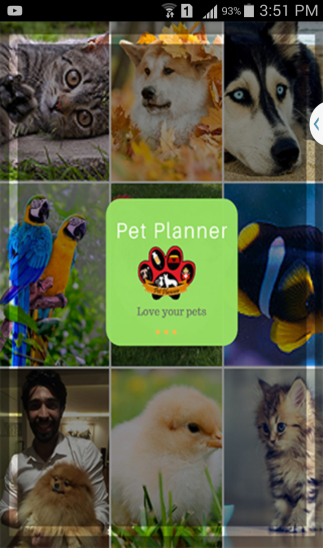
\includegraphics{00}
    \caption{Splash Screen}
\end{figure}

\newpage
\subsection{Login}

\begin{figure}[H]  
  \centering
    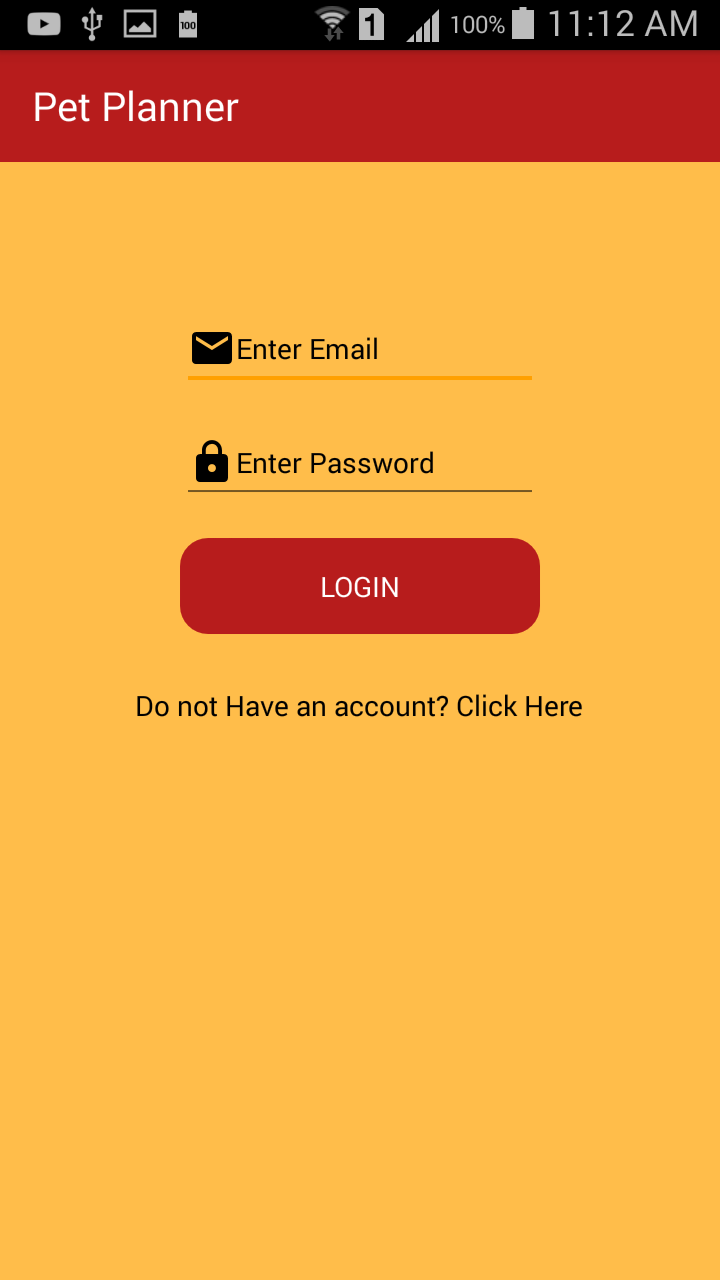
\includegraphics[scale=0.3]{81login}
    \caption{Login}
\end{figure}

User will enter valid email and password to login into the application.

\newpage
\subsection{Registration}
\begin{figure}[H]
  \centering
    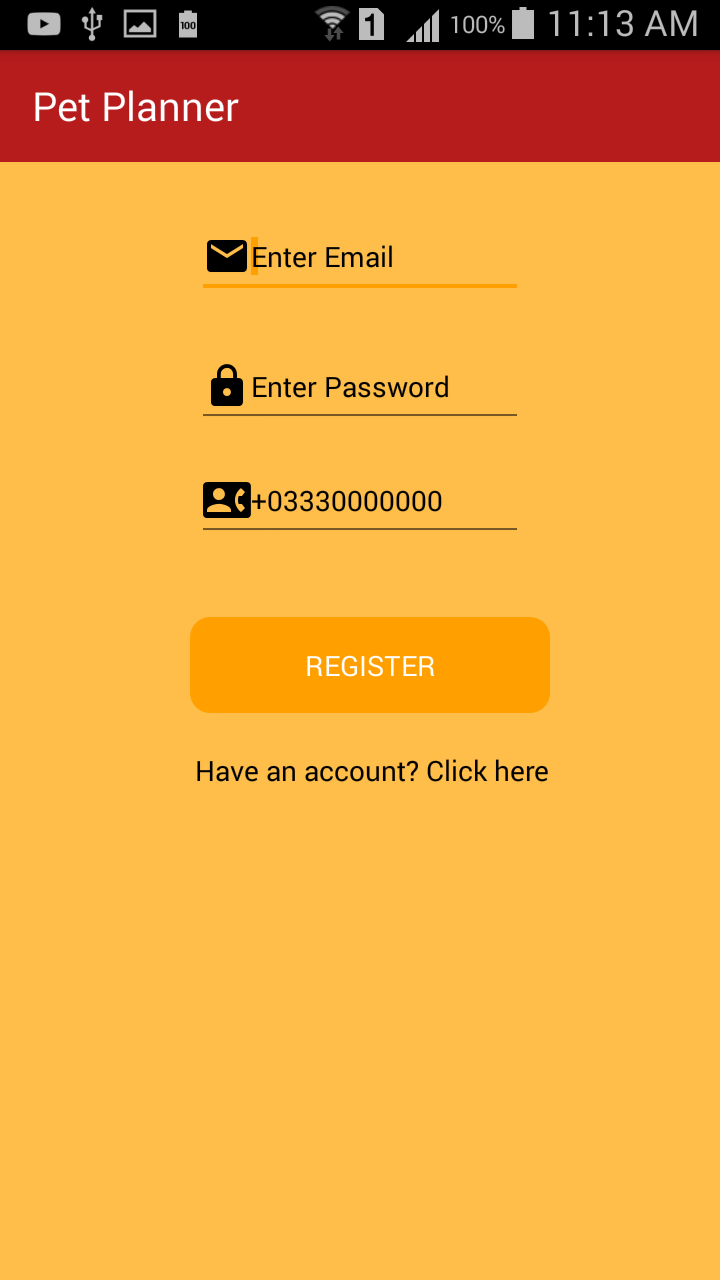
\includegraphics[scale=0.3]{82Registration}
     \caption{Registration}
\end{figure}

If user is new then he/she will register into the system.


\newpage
\subsection{Home Page}
\begin{figure}[H] 
  \centering
    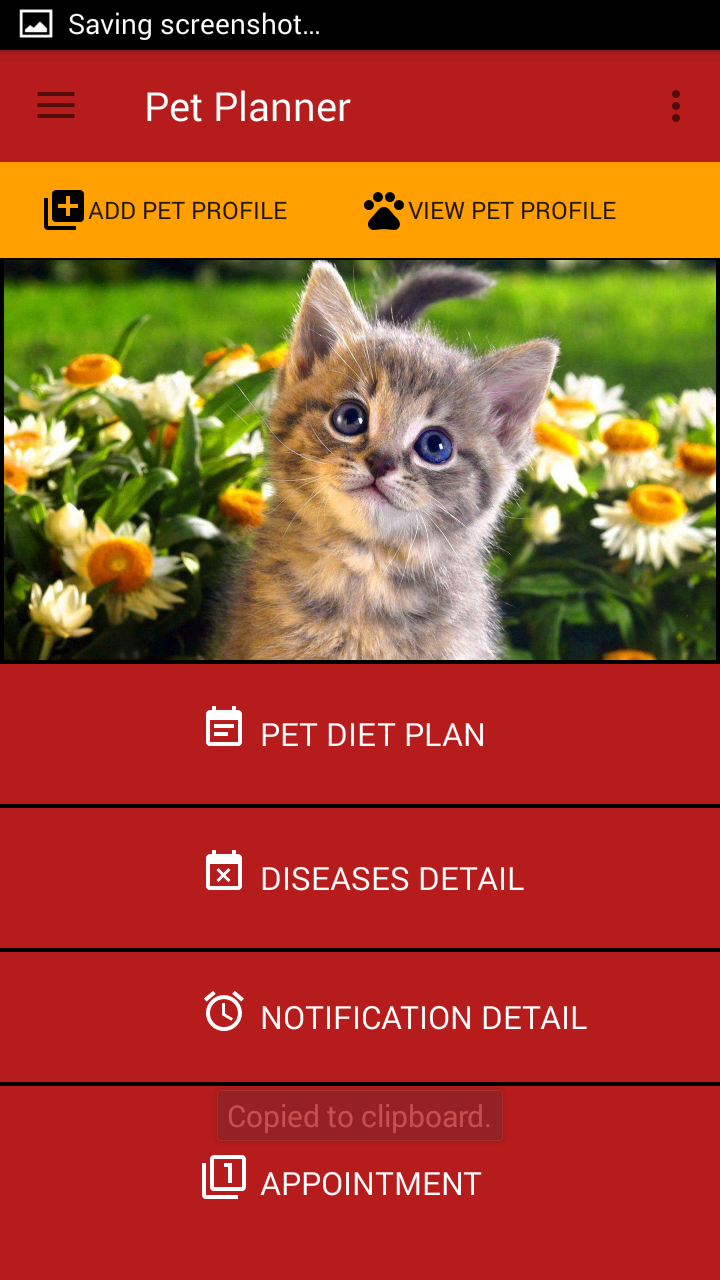
\includegraphics[scale=0.3]{89HomePage}
     \caption{Home Page}
\end{figure}
After the successful login user is able to add pet profile, view pet
 Profile, generate diet plan, view diseases details, generate alarm notifications and take appointment

\newpage
\subsection{Diet Plan}
\begin{figure}[H]
  \centering
    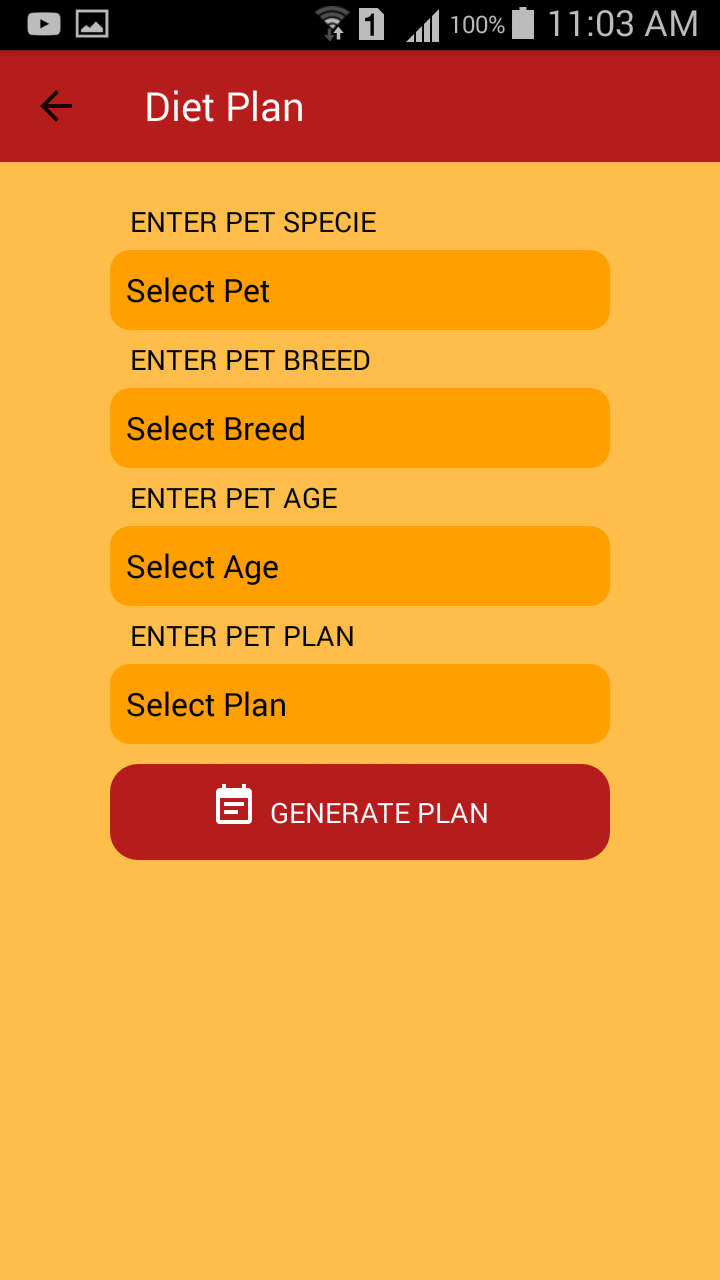
\includegraphics[scale=0.3]{86GenerateDietplan}
     \caption{Diet Plan}
\end{figure}

User can select pet specie, breed, age and plan to generate and download diet plan. 

\newpage
\subsection{Diseases Details}
\begin{figure}[H]
  \centering
    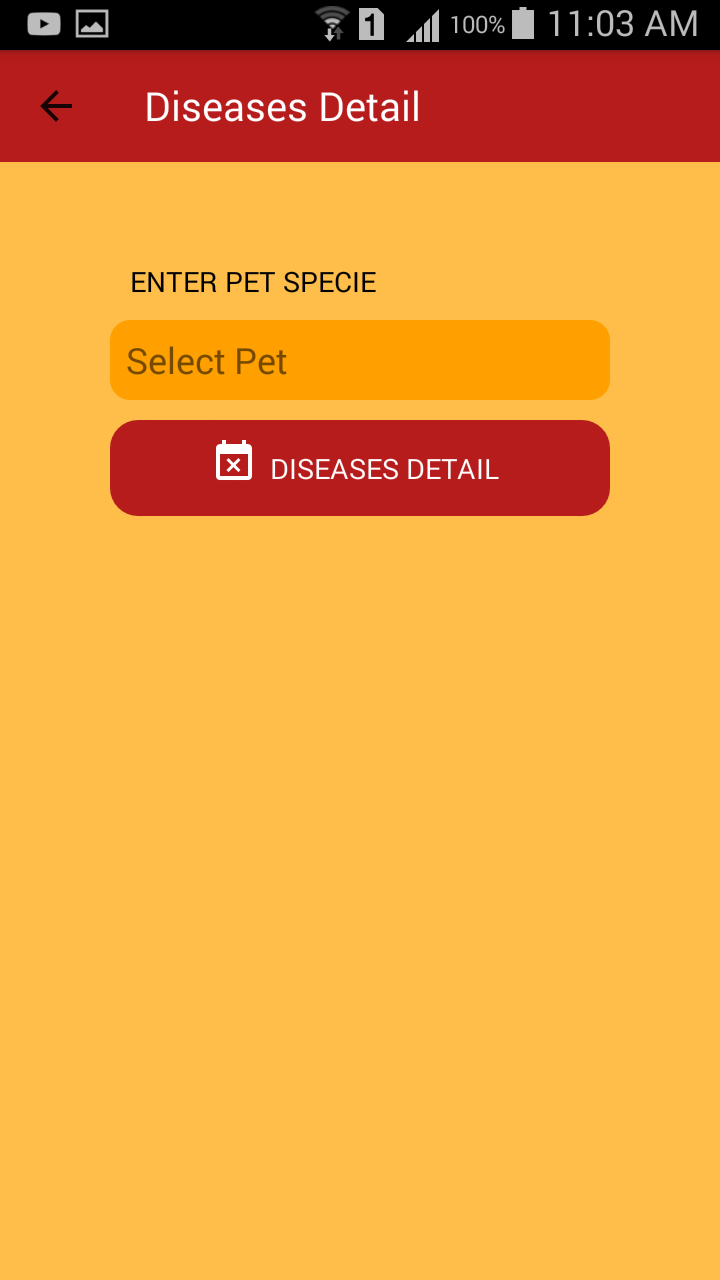
\includegraphics[scale=0.3]{87Diseases_Details}
     \caption{Diseases Details}
\end{figure}
User can select pet specie to view pet diseases details.

\newpage
\subsection{Notification Details}
\begin{figure}[H] 
  \centering
    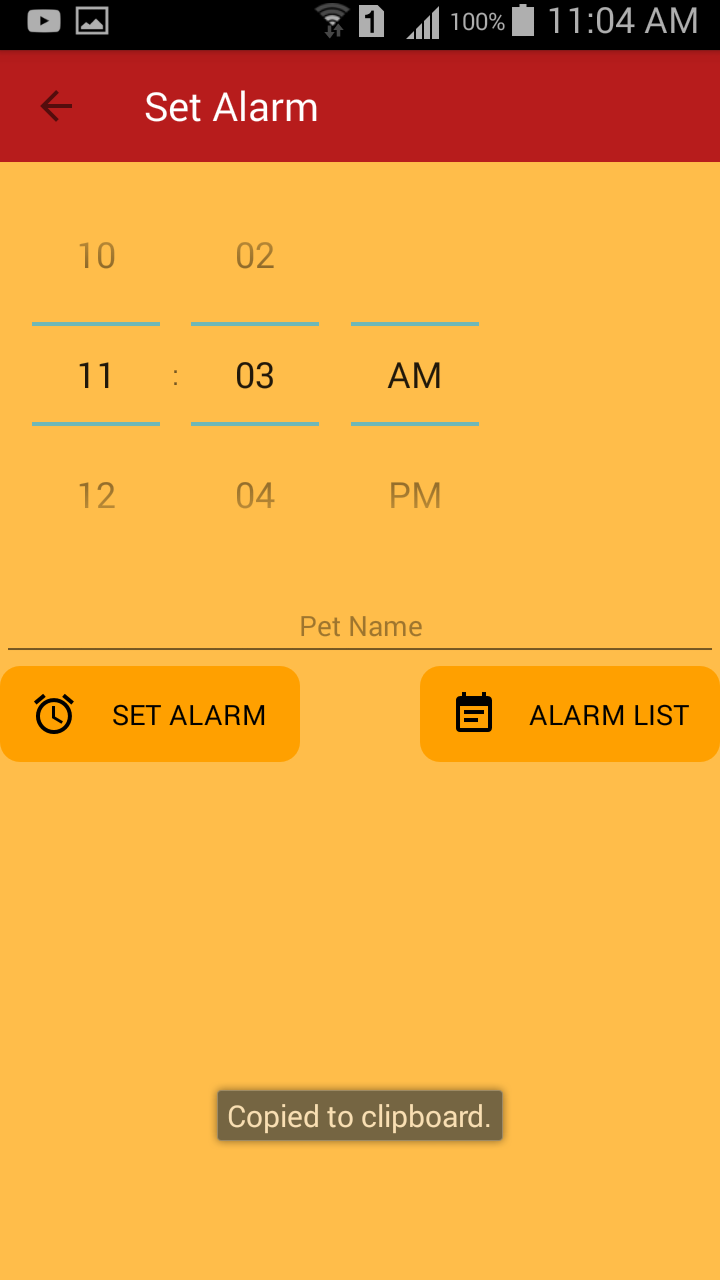
\includegraphics[scale=0.3]{85Alarmnotification}
    \caption{Notification Details}
\end{figure}

User can set alarm so that his pet could be feed.
\newpage
\subsection{Appointment}
\begin{figure}[H] 
  \centering
    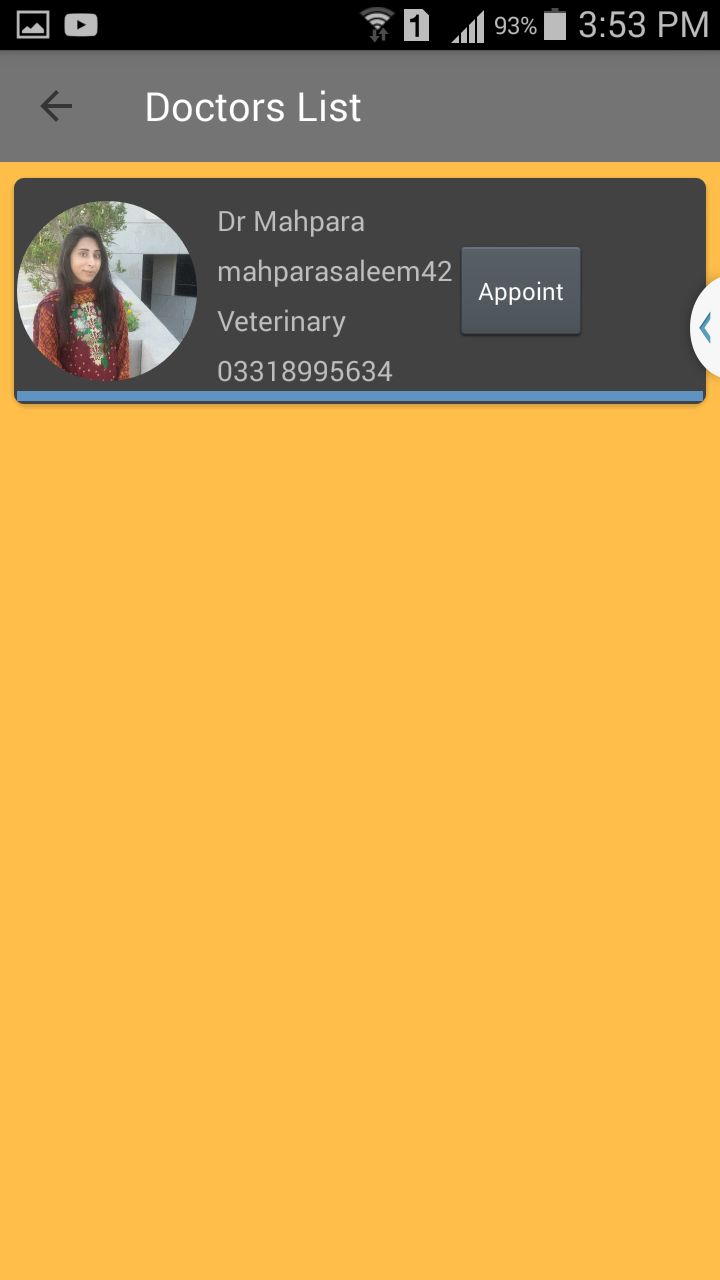
\includegraphics[scale=0.3]{88Appoint}
    \caption{Appointment}
\end{figure}

User can take appointment by clicking on Appoint button.
\newpage
\subsection{Add Pet Profile}
\begin{figure}[H] 
  \centering
    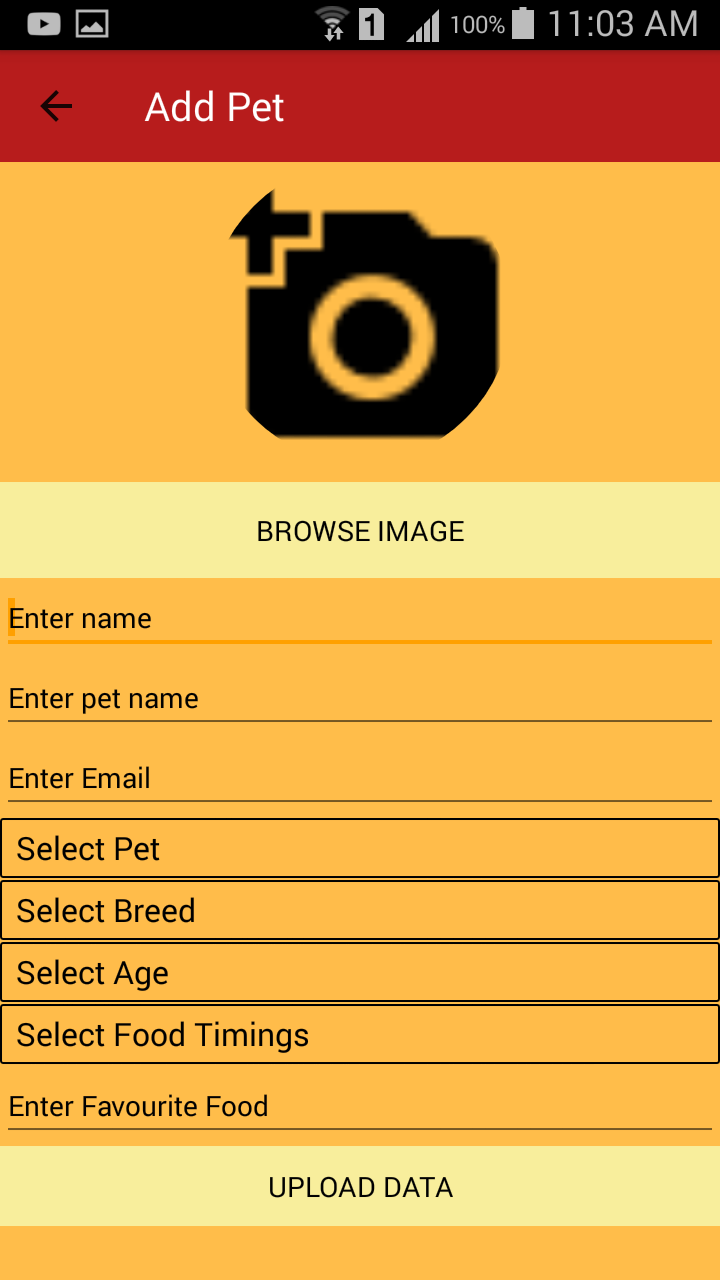
\includegraphics[scale=0.3]{83addpetprofile}
     \caption{Add Pet Profile}
\end{figure}
User can add pet details by filling all the fields.


\newpage
\subsection{View Pet Profile}

\begin{figure}[H]
  \centering
    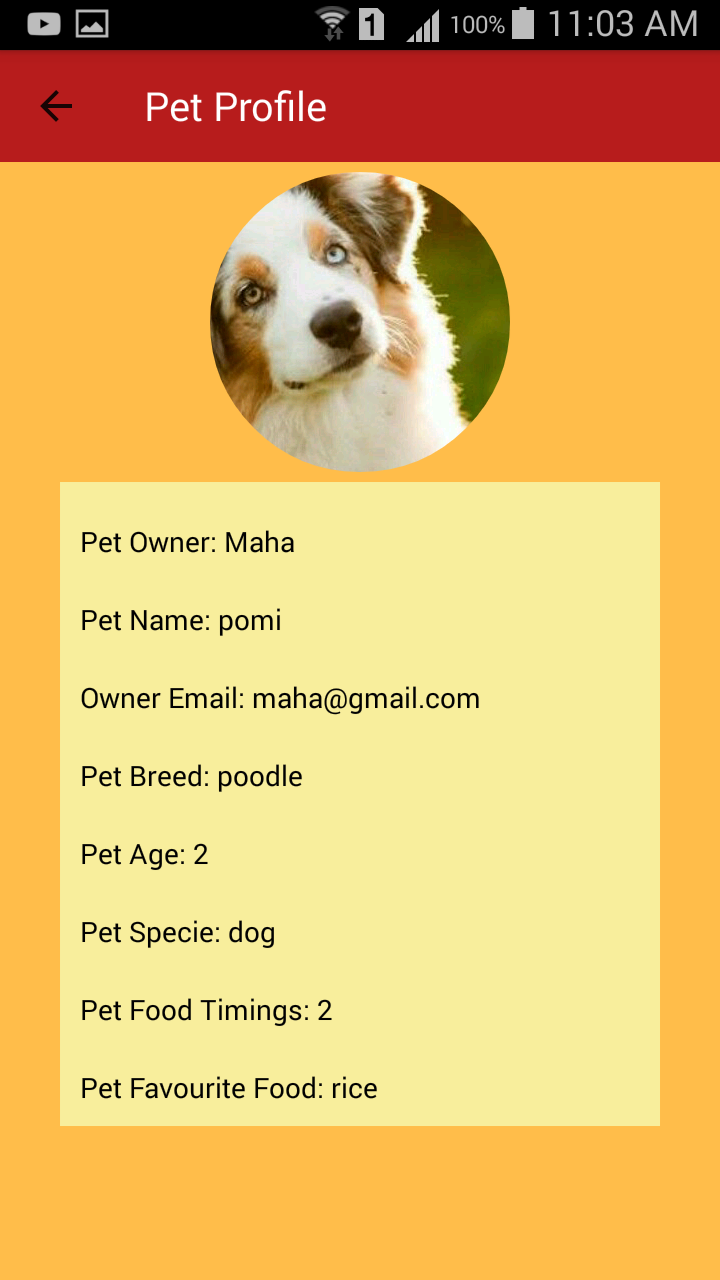
\includegraphics[scale=0.3]{84viewpetprofile}
      \caption{View Pet Profile}
\end{figure}

By clicking on view pet profile user is able to view pet profile.

\newpage
\subsection{Add as a Doctor}
\begin{figure}[H]
  \centering
    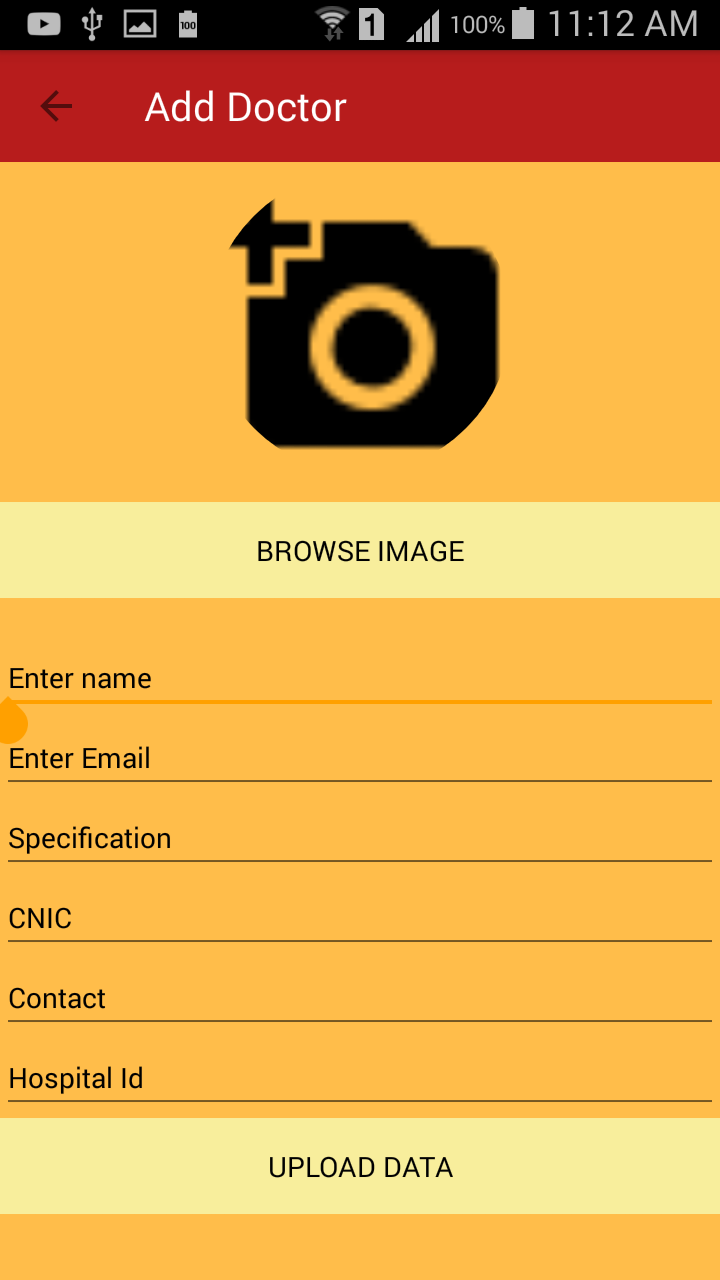
\includegraphics[scale=0.3]{90AddDoctorprofile}
      \caption{Add as a Doctor}
\end{figure}
Admin can be a doctor so he can register doctors by entering the correct hospital id assigned by the hospital to the doctor.


\chapter{Appendix} \label{ap:appendix2}

\section{Web Application}
\subsection{Home Button}
From Index page by clicking HOME will navigate to HOME screen.
\begin{figure}[H]
  \centering
    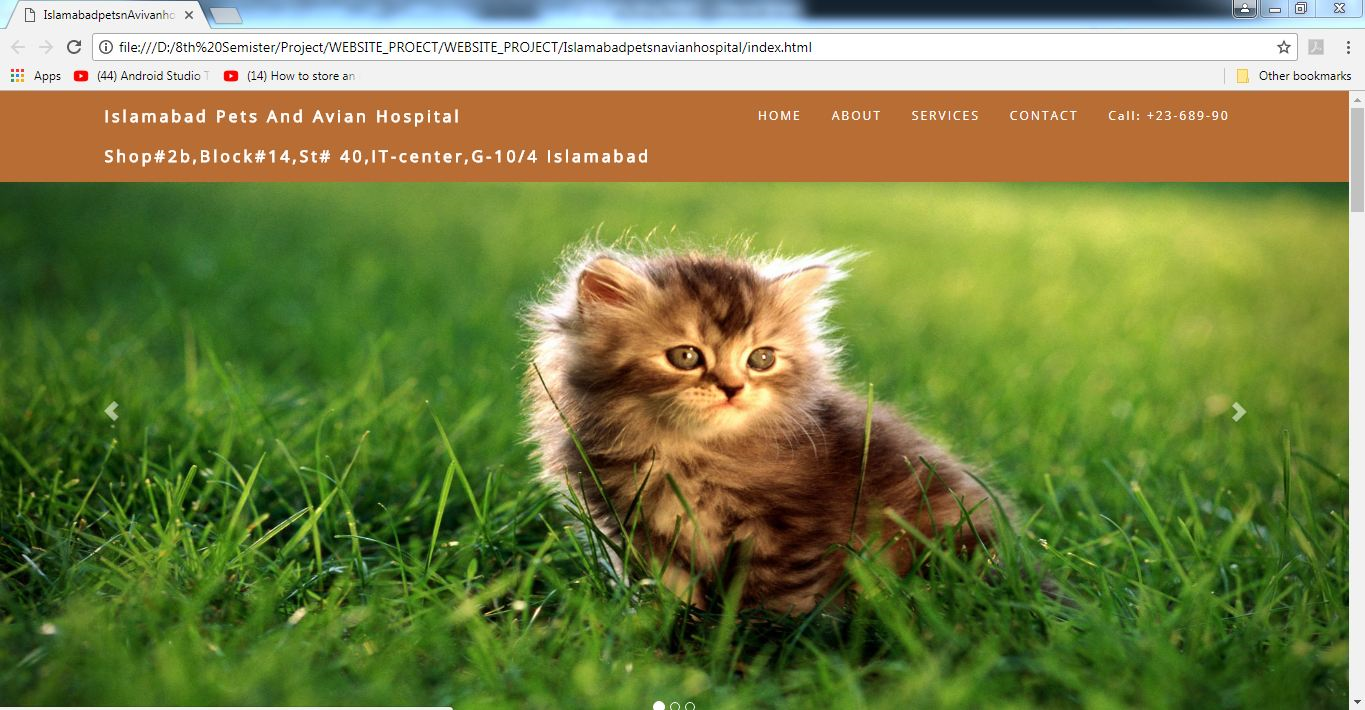
\includegraphics[scale=0.4]{appbone}
      \caption{Home}
\end{figure}

\newpage
\subsection{About us}
On selecting ABOUT from menu we navigate to ABOUT US screen
\begin{figure}[H]
  \centering
    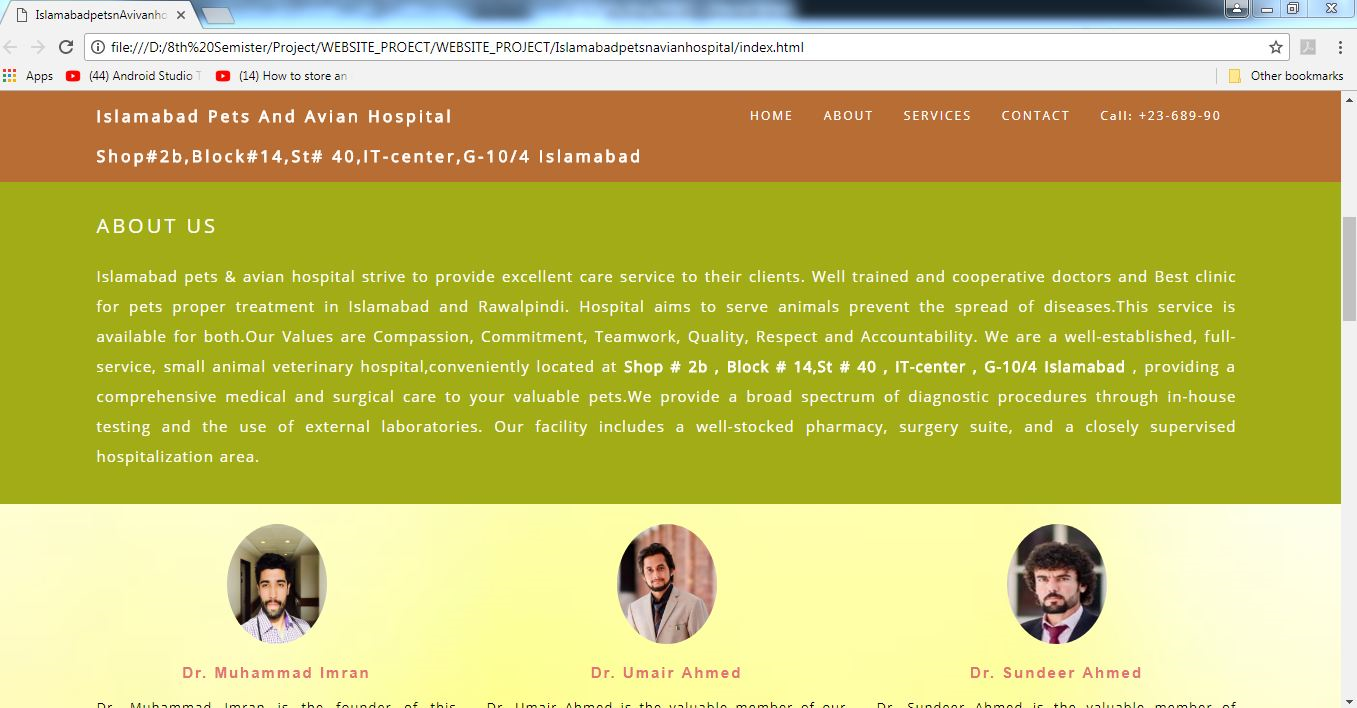
\includegraphics[scale=0.4]{aboutusapp}
     \caption{About Us}
\end{figure}


\subsection{Contact Us}
On selecting CONTACT from menu we navigate to CONTACT Screen.
\begin{figure}[H]
  \centering
    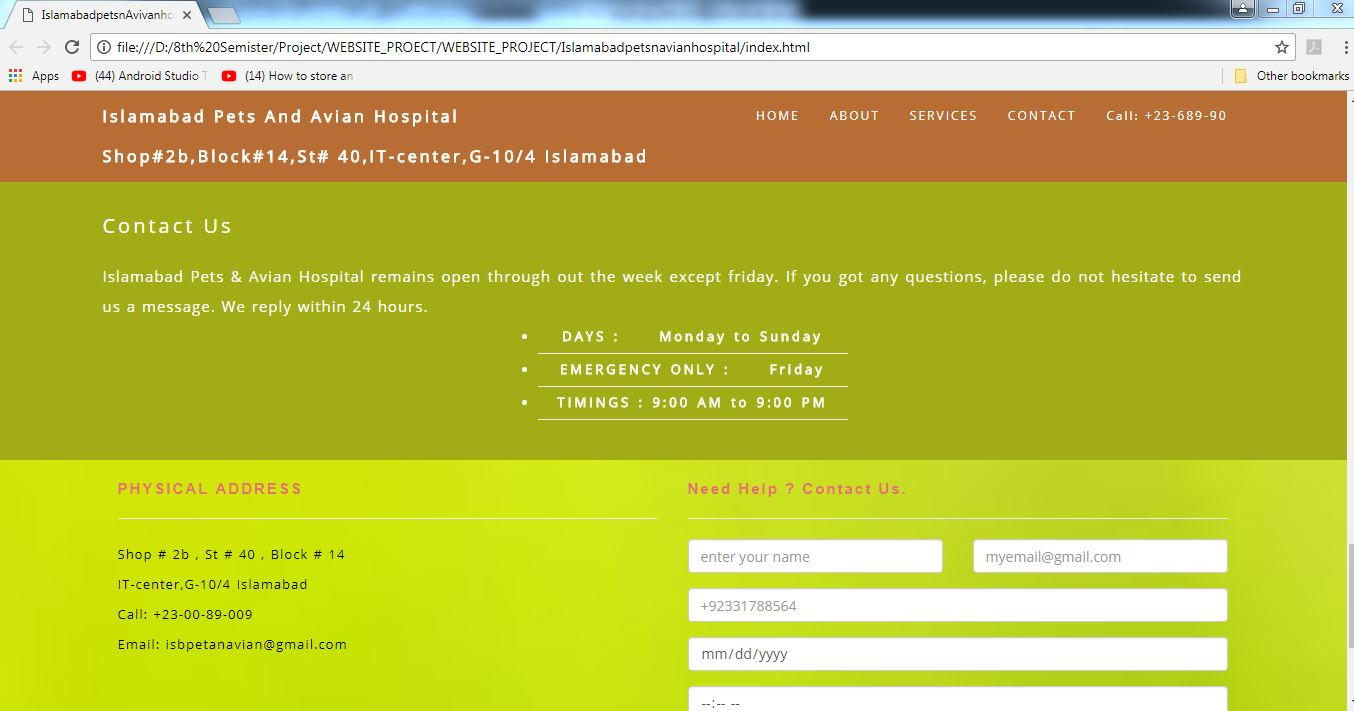
\includegraphics[scale=0.4]{contact}
     \caption{Contact us}
\end{figure}

\newpage
\subsection{Appointment}
User can take APPOINTMENT by full filling the entire field.
\begin{figure}[H]
  \centering
    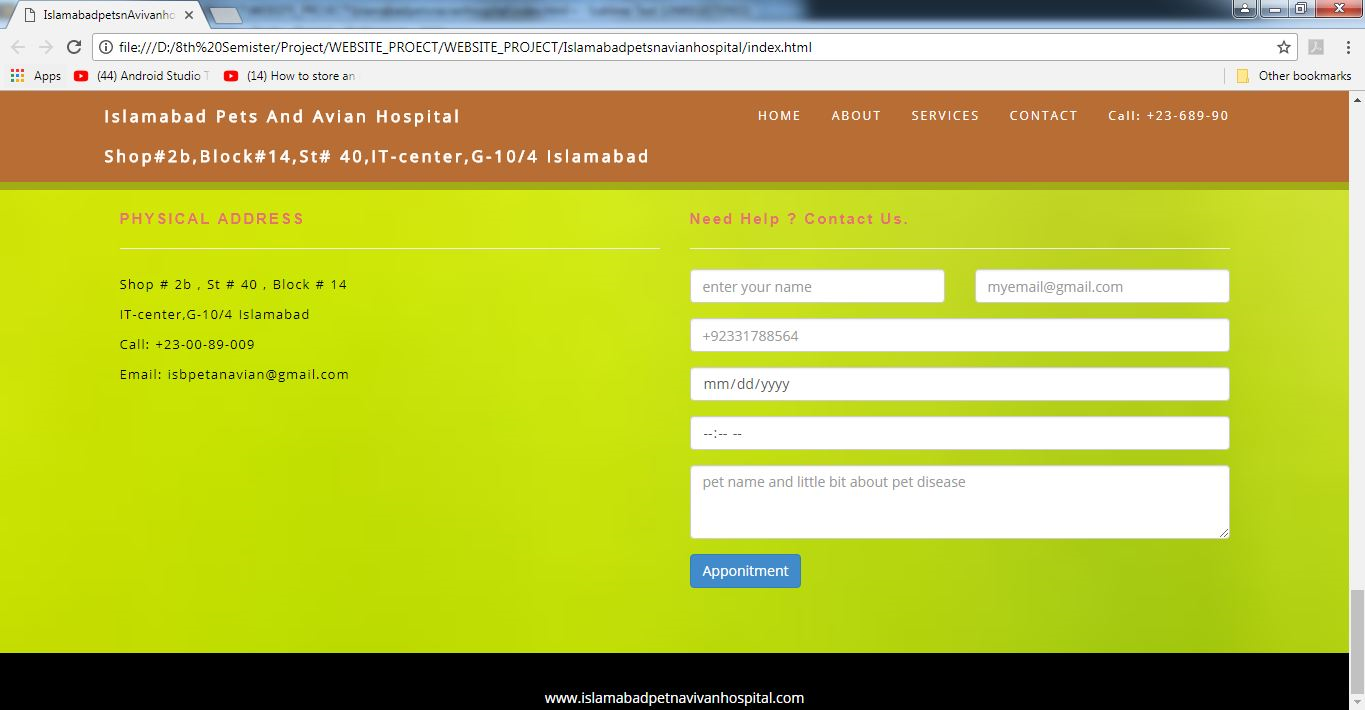
\includegraphics[scale=0.4]{appint}
     \caption{Appointment}
\end{figure}


















%%----------------------------------------
%% Final materials
%%----------------------------------------

\begin{singlespace}
  %% Bibliography
  %% comment the next command if BibTeX file not used
  %% bibliography is in ``references.bib''
  \PrintBib{references}

  %% Index
  %% uncomment next command if index is required
  %% don't forget to run ``makeindex tese'' command
  \PrintIndex
\end{singlespace}

\end{document}